%--------------------------------------------------------------------------
% Results
%--------------------------------------------------------------------------

\chapter{Results}
\label{cha: results}

\section{Temporal consistency of PALSAR mosaic data}
\label{sec: result-temporal-consistency}

Two sets of figures were used for analysing the distribution of radar backscatter vis-a-vis data acquisition dates. The first set consists of PALSAR mosaic data that were acquired in a single year but the data strips used to put the mosaic together were taken at different seasons; and the second consists of PALSAR mosaic data acquired along the same data strip or path but at different years.

\subsection{Mosaic data acquired in a single year but at different seasons}

Figs. \ref{fig: result-box4.1} and \ref{fig: result-box4.2} shows the distribution of backscatter values of forest cover types from PALSAR mosaic data acquired in a single year but at different seasons. The backscatter values of different forest types were plotted with respect to polarisation. Each mosaic is comprised of six strip data paths, particularly where there is land.

As an example, the figures in Fig. \ref{box: result-box4.3} show the 2007 PALSAR mosaic image and the dates of acquisition of each strip/path that comprise the whole mosaic (top), and the distribution of mean HH polarisation backscatter of each forest type based on the ROIs on the 2007 mosaic image (bottom). The images were taken from Fig. \ref{fig: method-fig3.6} and Figs. \ref{fig: result-box4.1} and \ref{fig: result-box4.2}, respectively. In the mosaic image, the dates of acquisition of the strips from left to right were taken at different months of the year, specifically: Jun 09, Jul 08, Sep 21, Oct 20, and Jun 16. Then, for the boxplots, the mean HH backscatter (y-axis) was plotted from the ROIs of each of the different forest cover types (x-axis), and under each forest cover type there can be a number of boxplots where each colour denotes the date of acquisition of the corresponding PALSAR strip data. For each box-whisker plot, the upper and lower hinges of the box correspond to the 1st and 3rd quartiles (25th and 75th percentiles). The band inside the box corresponds to the median (or the 2nd quartile). The upper whisker extends from the hinge to the highest value that is within 1.5 x IQR of the hinge, where IQR is the inter-quartile range, or distance between the 1st and 3rd quartiles. The lower whisker extends from the hinge to the lowest value within 1.5 x IQR of the hinge. Data beyond the end of the whiskers are outliers and are plotted as points.

The range of mean HH backscatter values fell between -2.50 dB and -11.25 dB across all forest cover types. It can be seen that for broadleaved forests, including closed and open canopy and forest plantation (FCFB, FOFB, FFPB), the mean HH backscatter values were recorded over four data strips/paths. Forest cover types with ROI samples recorded in three data strips/paths include open canopy coniferous forest (FOFC) and open canopy mixed forest (FOFM). The other forest types were distributed along only two data strips/paths, particularly: closed canopy coniferous forest (FCFC), closed canopy mixed forest (FCFM), and mangrove forest (LVMG), of which mangroves were only found along strip path data over coastlines. It should be noted that ROI samples for mangrove forest along the far left data strip/path (i.e., Jun 09) were not sufficient for plotting, hence the box-whisker plot was truncated. And finally, the coniferous forest plantation (FCFP) was recorded only within one data strip/path (i.e., Sep 21).

For FCFB, the ranges of mean backscatter values as shown by the boxplots generally overlapped (i.e., Jun 16, Aug 18, Sep 21), and hence can be considered temporally consistent, although the Oct 20 boxplot was slightly greater than the other plots. For FCFC and FCFM, boxplots denoting two adjacent data strips (i.e., Sep 21, Oct 20) also overlapped; hence their mean backscatter values can be treated as temporally consistent. For FFPB, three boxplots overlapped (i.e., Jul 08, Sep 21, Oct 20), which denote that their mean backscatter values can be considered temporally consistent. The Aug 18 boxplot shows lower mean backscatter, which can be attributed to low backscatter returning to the antenna due to karst substrate (i.e., Peñablanca Protected Landscape in Tuguegarao, Cagayan province) upon checking the locations of the ROIs found along the data strip. For FFPC, mean backscatter values were recorded on only one data strip (i.e., Sep 21). For FOFB, FOFC, and FOFM, all boxplots overlapped, indicating that mean backscatter values acquired over different months were within the same range, and hence were temporally consistent. For LVMG, the two boxplots overlapped (i.e., Jun 16, Aug 18), and hence their mean backscatter values can be considered as temporally consistent. Overall, the general overlaps shown by boxplots of each forest cover type suggest that the range of mean HH backscatter values over PALSAR mosaic data strips acquired in different months can be treated as temporally consistent.

Now looking at Figs. \ref{fig: result-box4.1} and \ref{fig: result-box4.2}, three plots are shown for each of the four years (hence, a total of 12 plots) that correspond to boxplots of mean HH backscatter, mean HV backscatter, and HH/HV ratio across the different forest cover types.

The mean HH backscatter of most forest types across four years (2007-2010) was approximately between -2.50 dB to -11.25 dB in terms of their minimum and maximum values, indicating values were generally consistent across different seasons. For mangrove forest (LVMG), the backscatter values were approximately below -5.0 dB. Broadleaved forests, both closed and open canopy (FCFB, FOFB), exhibited narrow ranges denoting lower variability, and their median values were also generally consistent at the same level and did not vary across different seasons or different years.

The mean HV backscatter of most forest types across four years was approximately between -7.50 dB to -17.50 dB in terms of their minimum and maximum values, also indicating that values were generally consistent across different seasons within mosaic image acquired within a single year. Mangrove forest (LVMG) backscatter values were approximately between -11.0 dB and -17.5 dB, and generally had lower backscatter values compared to other forest cover types (notably the 25th to 75th percentile range of boxplots). Similar to mean HH backscatter, broadleaved forests, both closed and open canopy (FCFB, FOFB), also exhibited narrow ranges denoting lower variability, and their median values were also generally consistent at the same level and did not vary across different seasons or different years.

For the mean HH/HV ratio plots, values were approximately from 1.5 to 2.5 for all forest types (excluding outliers). Mangrove forest (LVMG) exhibited higher median values, generally observed at 2.0 and above, compared to other forest types that had values from 1.5 to 2.0.

\subsection{Mosaic data acquired along one path of strip data but across different years}

Figure 13 shows the distribution of backscatter values of forest cover types from PALSAR mosaic data from only one path of strip data but across different years. Similar to Figure 12, the backscatter values of different forest types were also plotted with respect to polarisation, and each mosaic is comprised of six strip data paths, particularly where there is land.

As an example, the figures in Fig. \ref{box: result-box4.4} show the one of the PALSAR regional mosaics with a highlight along the specific strip/path where ROIs of forest cover types were taken across different years, specifically from 2007 to 2010 (top), and the distribution of mean HH polarisation backscatter of each forest type along the same strip/path at different years (bottom). The images were taken from Fig. \ref{fig: method-fig3.6} and Figure 13, respectively. The dates of acquisition along the same strip/path taken at different years were: 21 Sep 2007, 08 May 2008, 26 Jun 2009, and 29 Jun 2010. Then, for the boxplots, the mean HH backscatter (y-axis) was plotted from the ROIs of each of the different forest cover types (x-axis), except for mangrove forest (LVMG) since there were no mangroves present within the data strip. Under each forest cover type there can be a number of boxplots where each colour denotes the date of acquisition along the same strip at different years.

The range of mean HH backscatter values fell between -2.50 dB and -11.25 dB across all forest cover types across different years. Median values of mean HH backscatter at different years consistently overlapped for each forest cover type, except for some very slight fluctuations. Overall, the overlaps shown by boxplots of each forest cover type suggest that the range of mean HH backscatter values over the same PALSAR mosaic data strip acquired in different years can be considered as temporally consistent.

Now looking at Figure 13, three plots are shown for each of the two highlighted data strips/paths that correspond to boxplots of mean HH backscatter, mean HV backscatter, and HH/HV ratio across the different forest cover types. Backscatter values were assessed for two different data strips/paths: one in Cordillera (Strip 1) and the other in Sierra Madre (Strip 2). Eight forest types were present along the Cordillera strip (except mangrove forest) while four forest types were present in the Sierra Madre strip (except coniferous and mixed forest types).

For the Cordillera data strip (Strip 1), the mean HH backscatter values were approximately from -2.5 dB to -10.0 dB, while the mean HV backscatter values were approximately from -7.5 dB to -15.0 dB. Median values were at consistent levels across different years for each forest type. The mean HH/HV ratio values were generally from 1.0 to 2.0 with consistent median values across different years for each forest type. For the Sierra Madre data strip (Strip 2), the mean HH backscatter values were approximately from -5.0 dB to -10.0 dB, while the mean HV backscatter values were approximately from -10.0 dB to -17.5 dB, of which mangrove forest (LVMG) had lower values compared to broadleaved forest types. Median values were generally at consistent levels across different years for each forest type. The mean HH/HV ratio values were also generally from 1.0 to 2.0, except for mangrove forest with values of 2.0 and above.

Overall, the distribution of mean backscatter of forest cover types for both HH and HV polarisation overlapped. The values of forest cover types in HH/HV ratio also overlapped, except for mangrove forest (LVMG), which had slightly higher values compared to other forest types. This emphasises that these forest types cannot be discriminated using solely polarimetric data.

The backscatter analysis demonstrated that the ALOS/PALSAR mosaics were temporally consistent despite the difference in seasons of acquisition dates of the strip data (usually within a range of 3-5 months) or the difference in annual dates of acquisition.

\begin{landscape}
\begin{figure}[!ht] \centering
	\captionsetup[subfigure]{width=2.0in} % <-- Use this to control text which is poorly spaced under a subfigure. 
	\begin{subfigure}[t]{0.43\textwidth}
		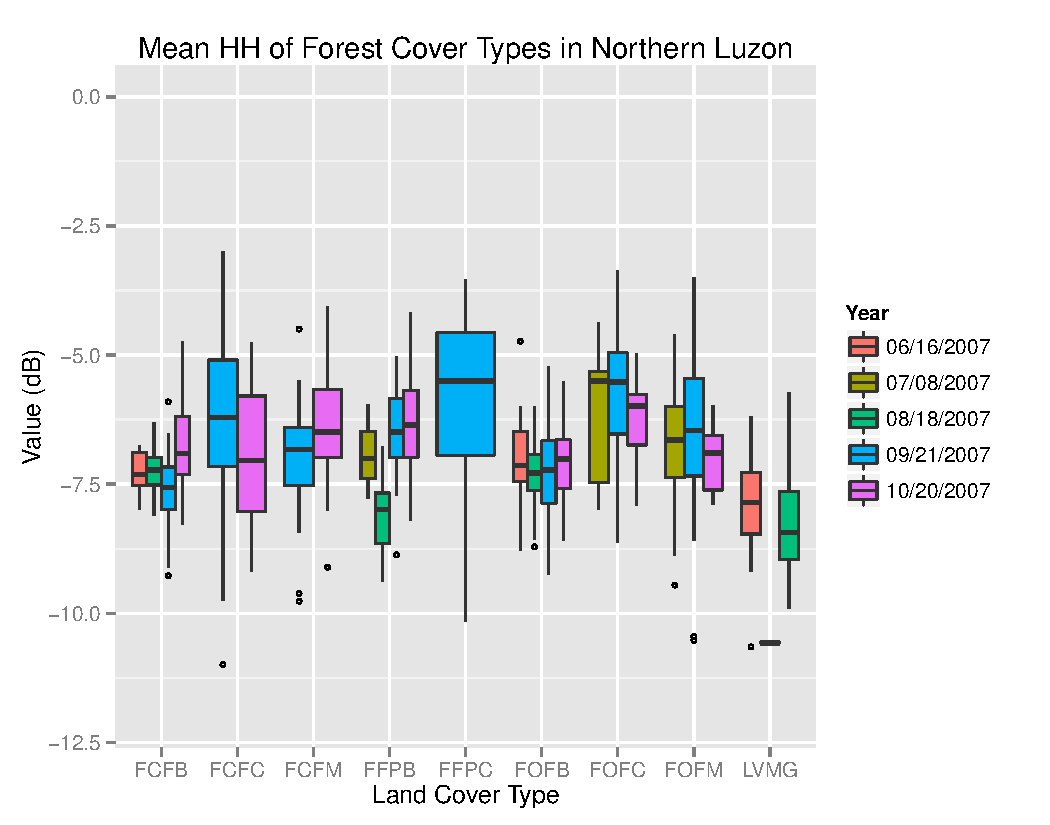
\includegraphics[width=\textwidth]{fig_boxplot-2007-mean-hh.pdf}
		\caption[Single year backscatter boxplots.]{2007 Mean HH.}
		\label{fig: result-box4.1a}
	\end{subfigure}
	\begin{subfigure}[t]{0.43\textwidth}
		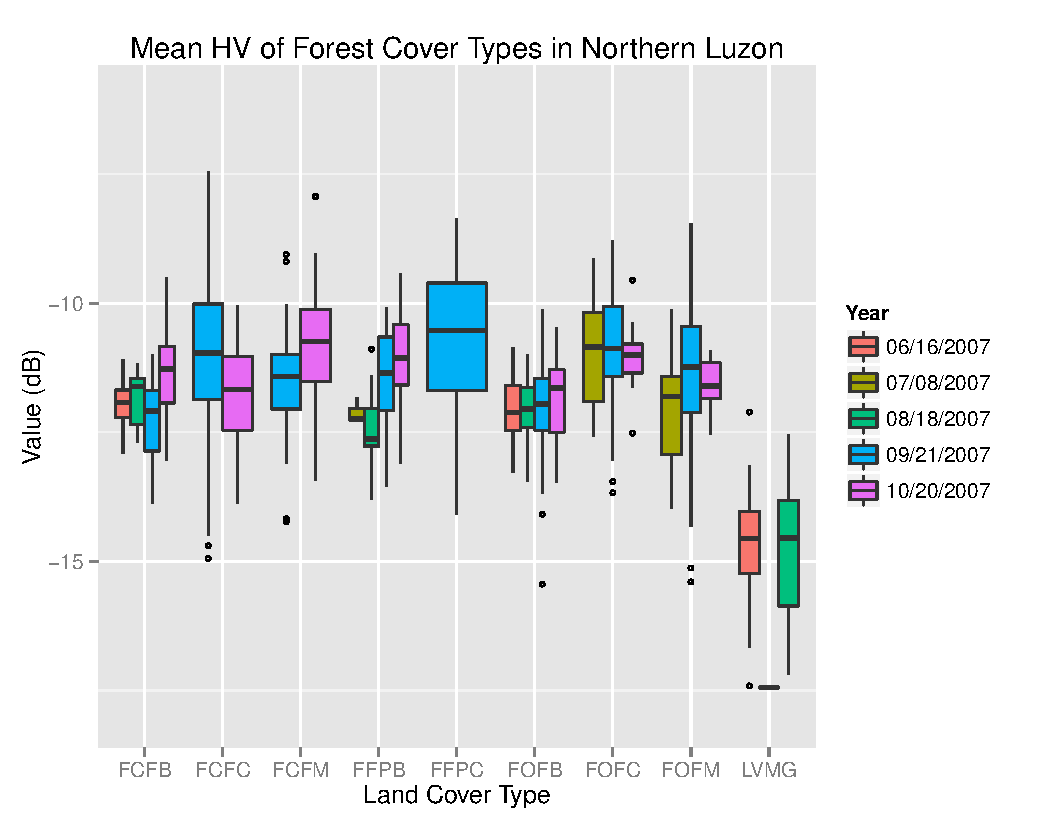
\includegraphics[width=\textwidth]{fig_boxplot-2007-mean-hv.pdf}
		\caption[Single year backscatter boxplots.]{2007 Mean HV.}
		\label{fig: result-box4.1b}
	\end{subfigure}
	\begin{subfigure}[t]{0.43\textwidth}
		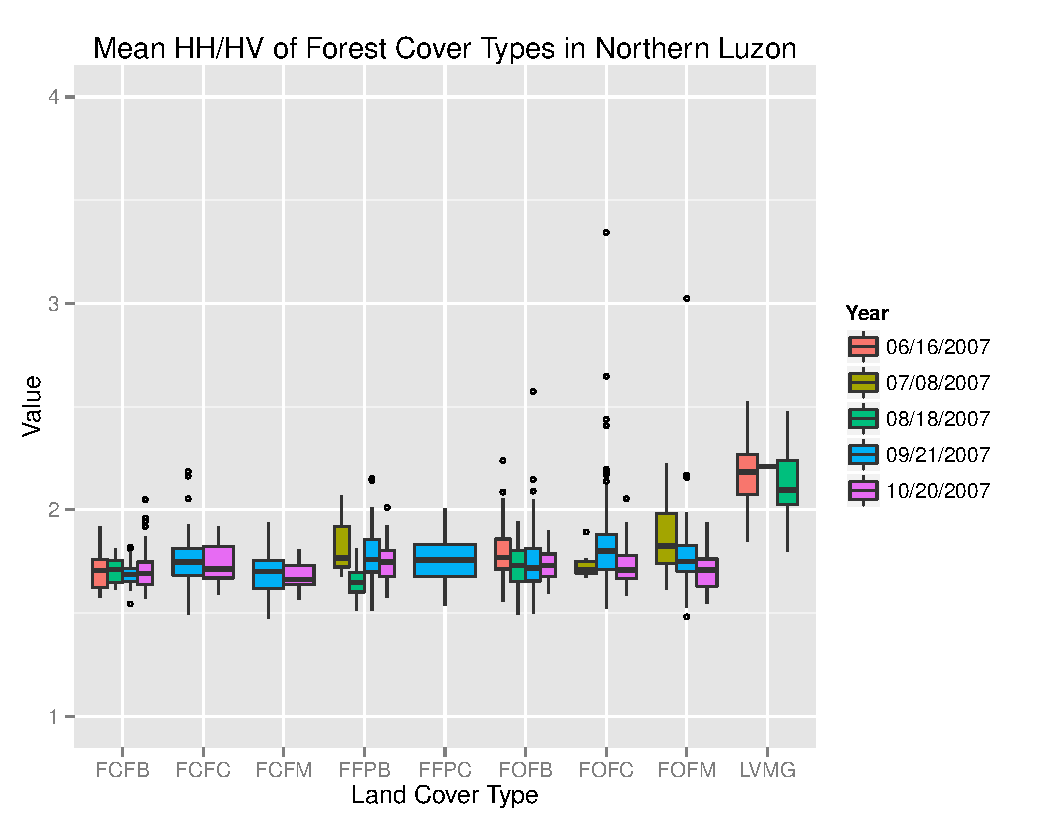
\includegraphics[width=\textwidth]{fig_boxplot-2007-mean-rat.pdf}
		\caption[Single year backscatter boxplots.]{2007 Mean HH/HV.}
		\label{fig: result-box4.1c}
	\end{subfigure}\\
	\vspace{20pt}
	\begin{subfigure}[t]{0.43\textwidth}
		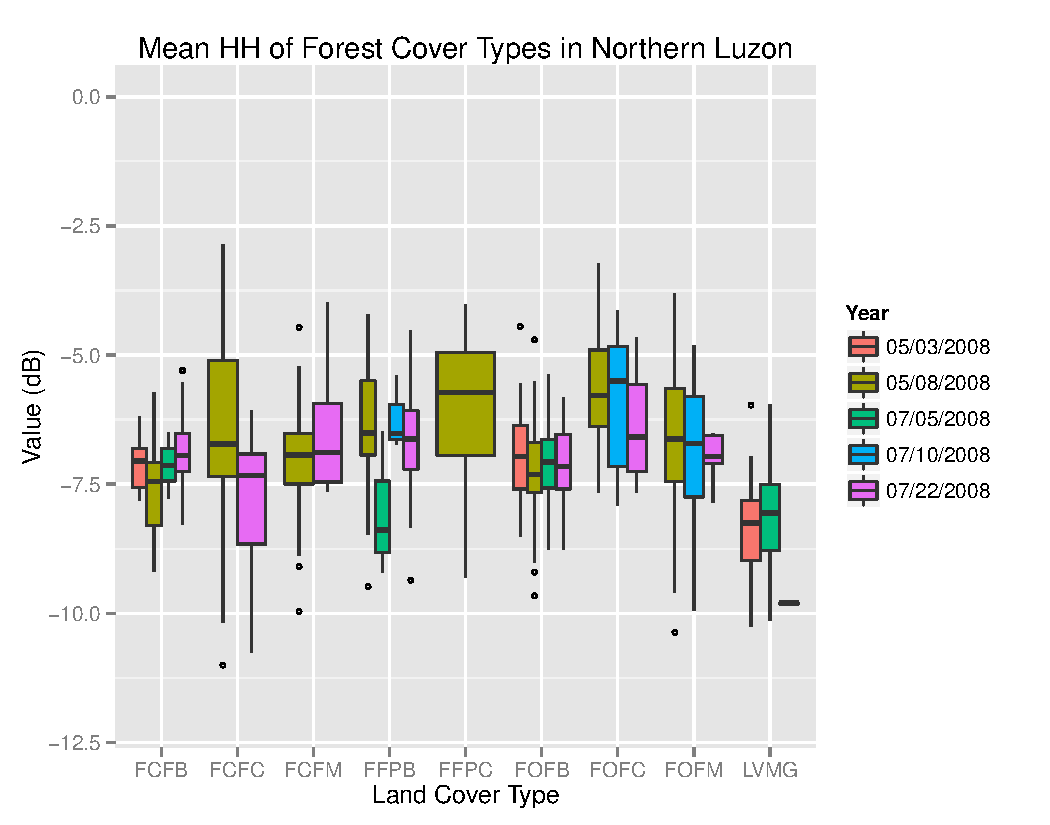
\includegraphics[width=\textwidth]{fig_boxplot-2008-mean-hh.pdf}
		\caption[Single year backscatter boxplots.]{2008 Mean HH.}
		\label{fig: result-box4.1d}
	\end{subfigure}
	\begin{subfigure}[t]{0.43\textwidth}
		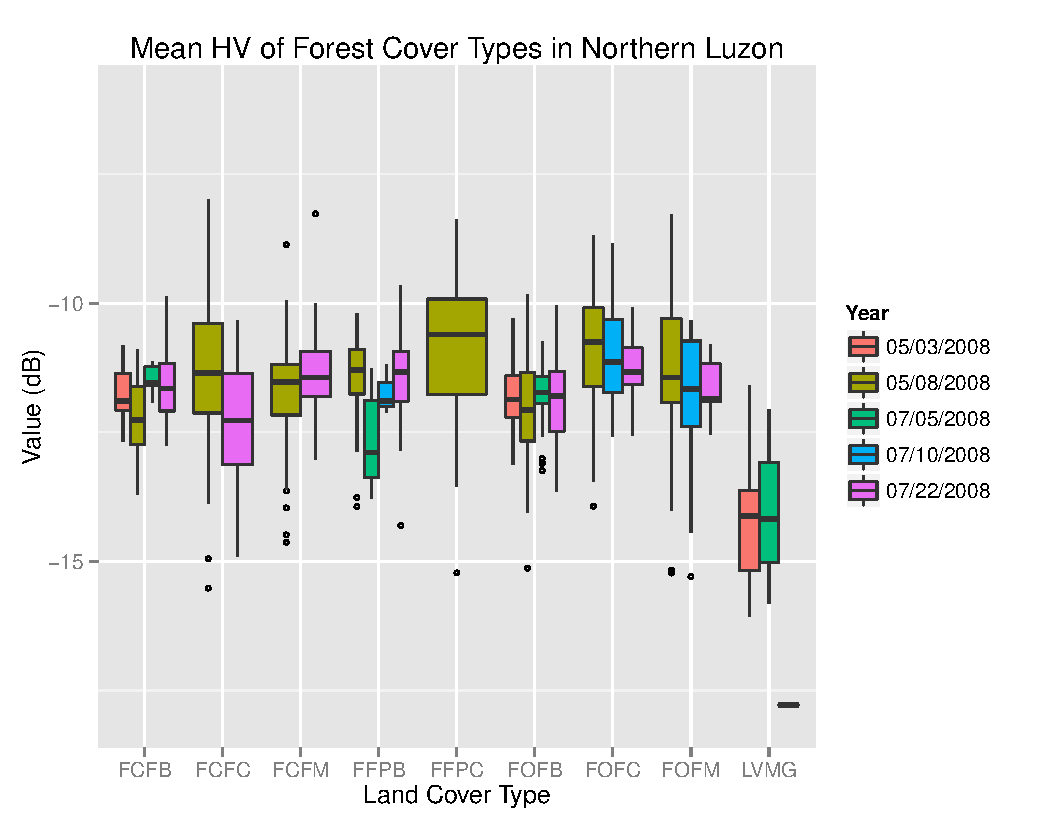
\includegraphics[width=\textwidth]{fig_boxplot-2008-mean-hv.pdf}
		\caption[Single year backscatter boxplots.]{2008 Mean HV.}
		\label{fig: result-box4.1e}
	\end{subfigure}
	\begin{subfigure}[t]{0.43\textwidth}
		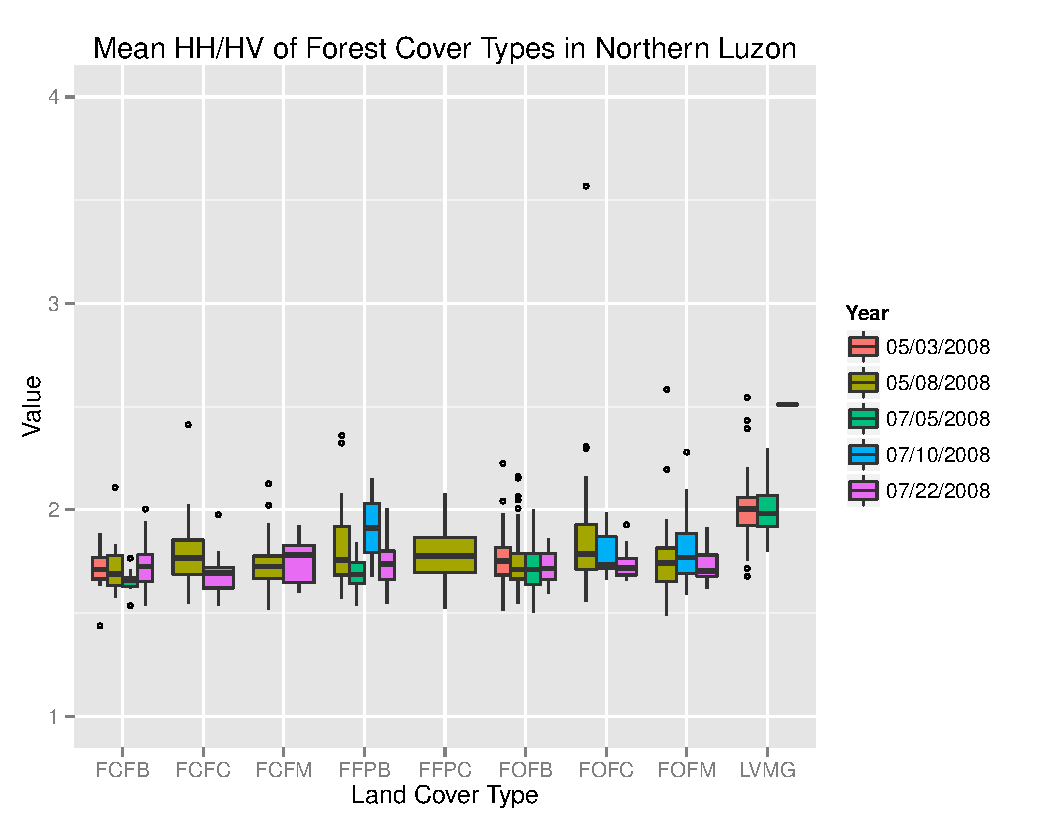
\includegraphics[width=\textwidth]{fig_boxplot-2008-mean-rat.pdf}
		\caption[Single year backscatter boxplots.]{2008 Mean HH/HV.}
		\label{fig: result-box4.1f}
	\end{subfigure}\\
	\vspace{20pt}
	\caption[Backscatter values of forest types from PALSAR data acquired in a single year at different seasons.]{Backscatter values of forest types from PALSAR data acquired in a single year at different seasons. Shown are box-whisker plots of mean backscatter values in 2007 (a-c) and 2008 (d-f).}
	\label{fig: result-box4.1}
\end{figure}
\end{landscape}

\begin{landscape}
\begin{figure}[!ht] \centering
	\captionsetup[subfigure]{width=2.0in} % <-- Use this to control text which is poorly spaced under a subfigure. 
	\begin{subfigure}[t]{0.43\textwidth}
		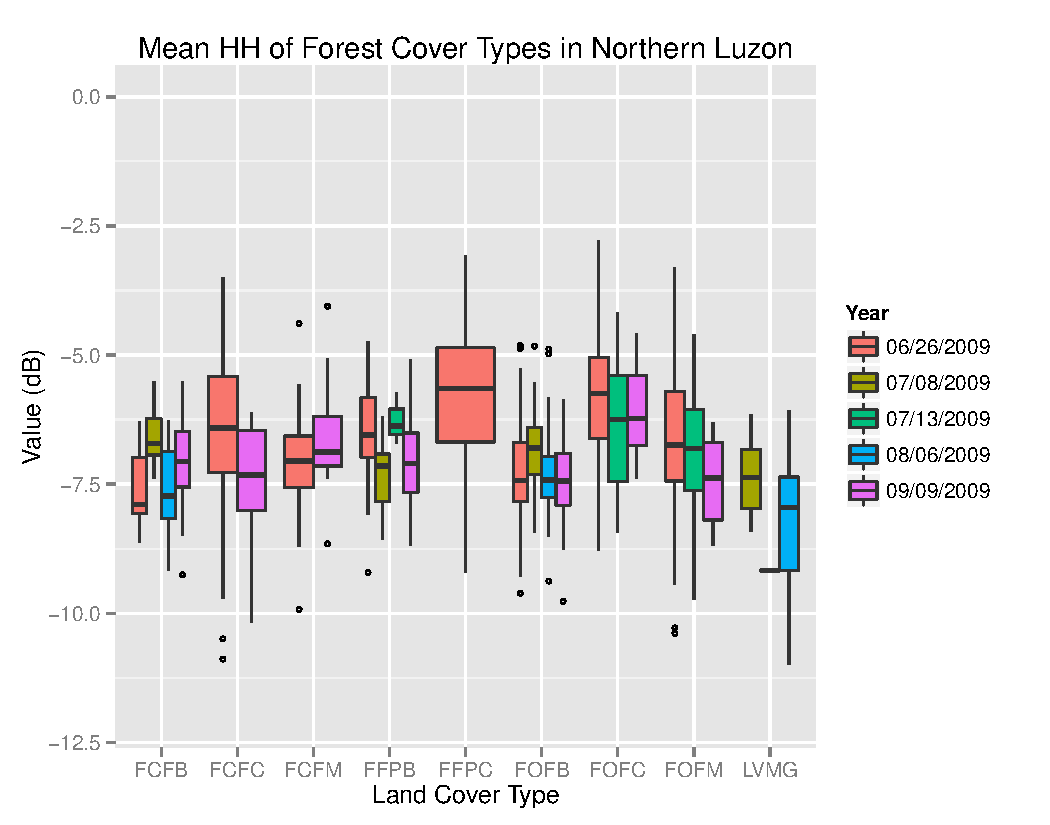
\includegraphics[width=\textwidth]{fig_boxplot-2009-mean-hh.pdf}
		\caption[Single year backscatter boxplots.]{2009 Mean HH.}
		\label{fig: result-box4.2a}
	\end{subfigure}
	\begin{subfigure}[t]{0.43\textwidth}
		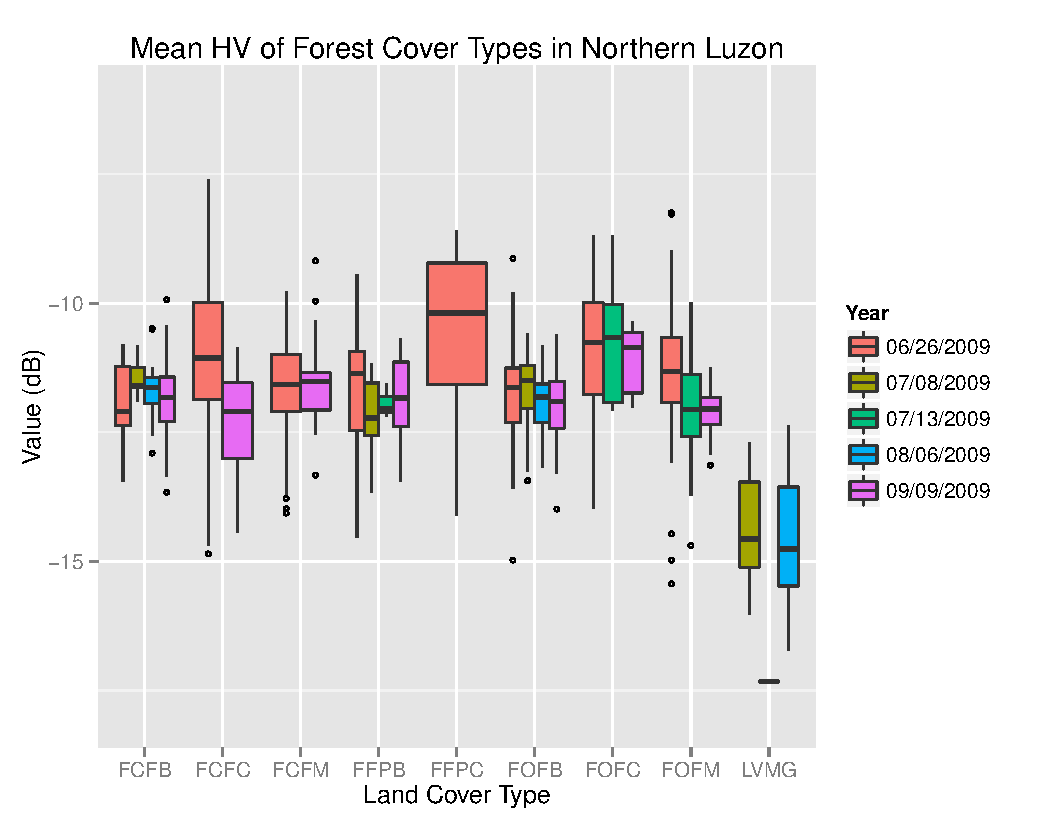
\includegraphics[width=\textwidth]{fig_boxplot-2009-mean-hv.pdf}
		\caption[Single year backscatter boxplots.]{2009 Mean HV.}
		\label{fig: result-box4.2b}
	\end{subfigure}
	\begin{subfigure}[t]{0.43\textwidth}
		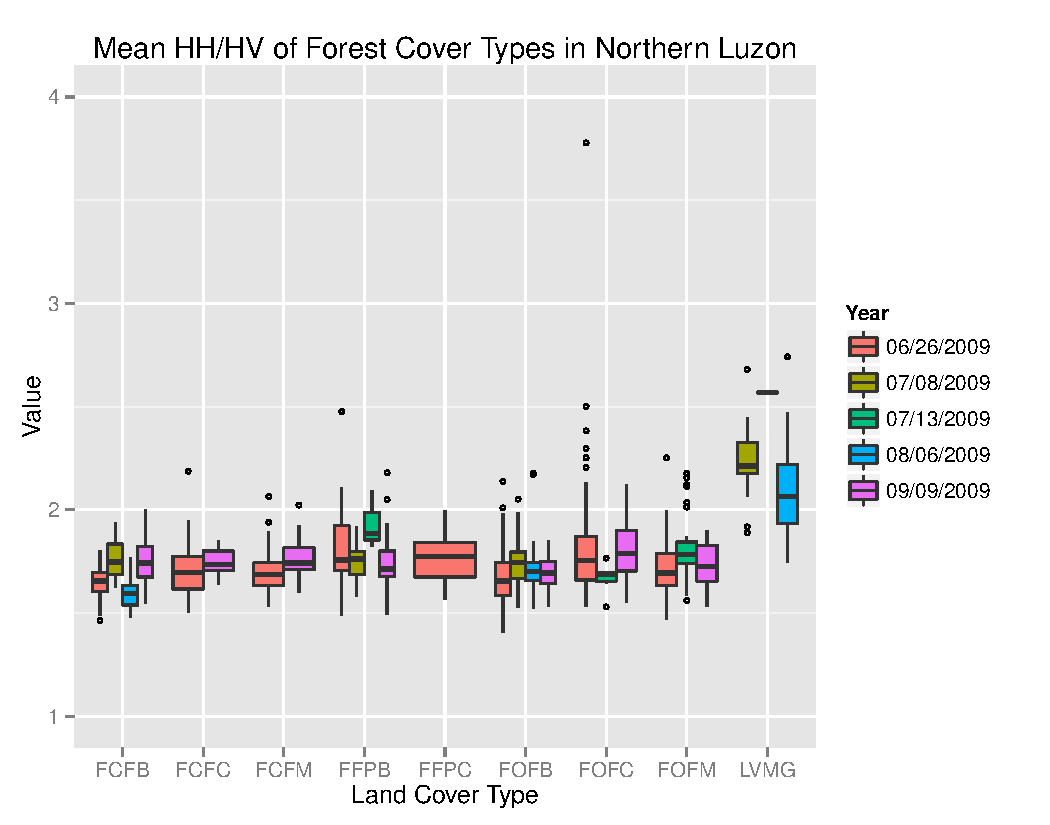
\includegraphics[width=\textwidth]{fig_boxplot-2009-mean-rat.pdf}
		\caption[Single year backscatter boxplots.]{2009 Mean HH/HV.}
		\label{fig: result-box4.2c}
	\end{subfigure}\\
	\vspace{20pt}
	\begin{subfigure}[t]{0.43\textwidth}
		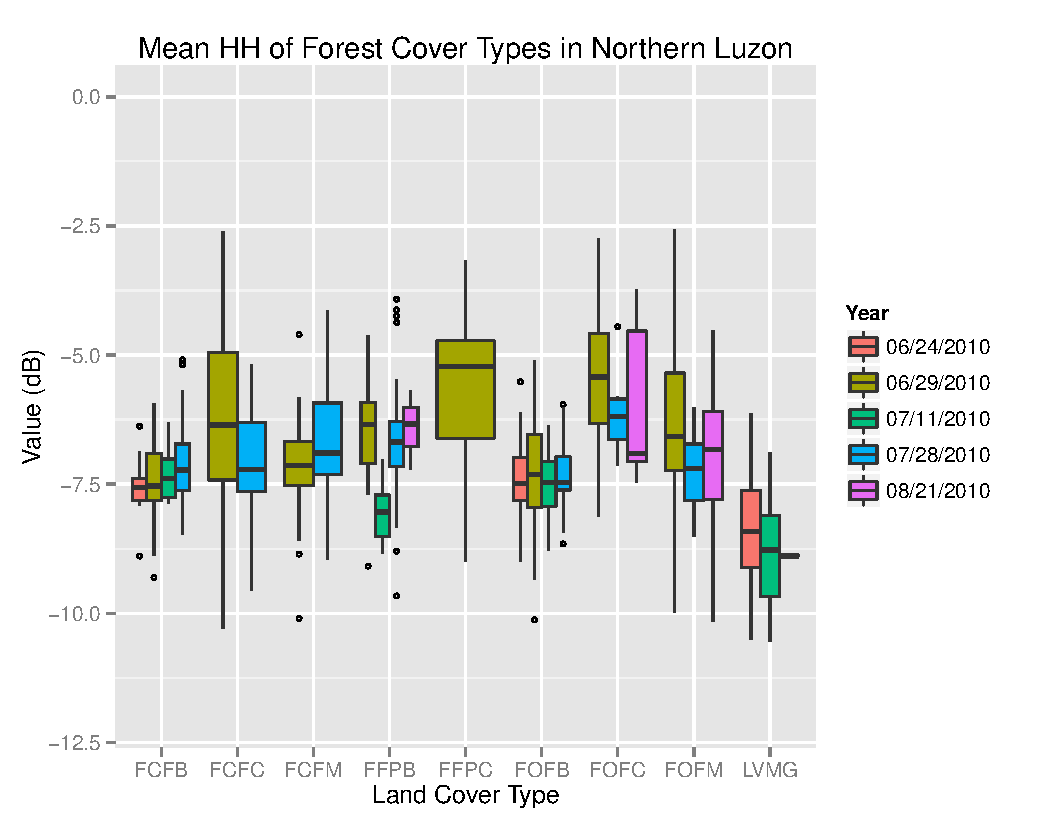
\includegraphics[width=\textwidth]{fig_boxplot-2010-mean-hh.pdf}
		\caption[Single year backscatter boxplots.]{2010 Mean HH.}
		\label{fig: result-box4.2d}
	\end{subfigure}
	\begin{subfigure}[t]{0.43\textwidth}
		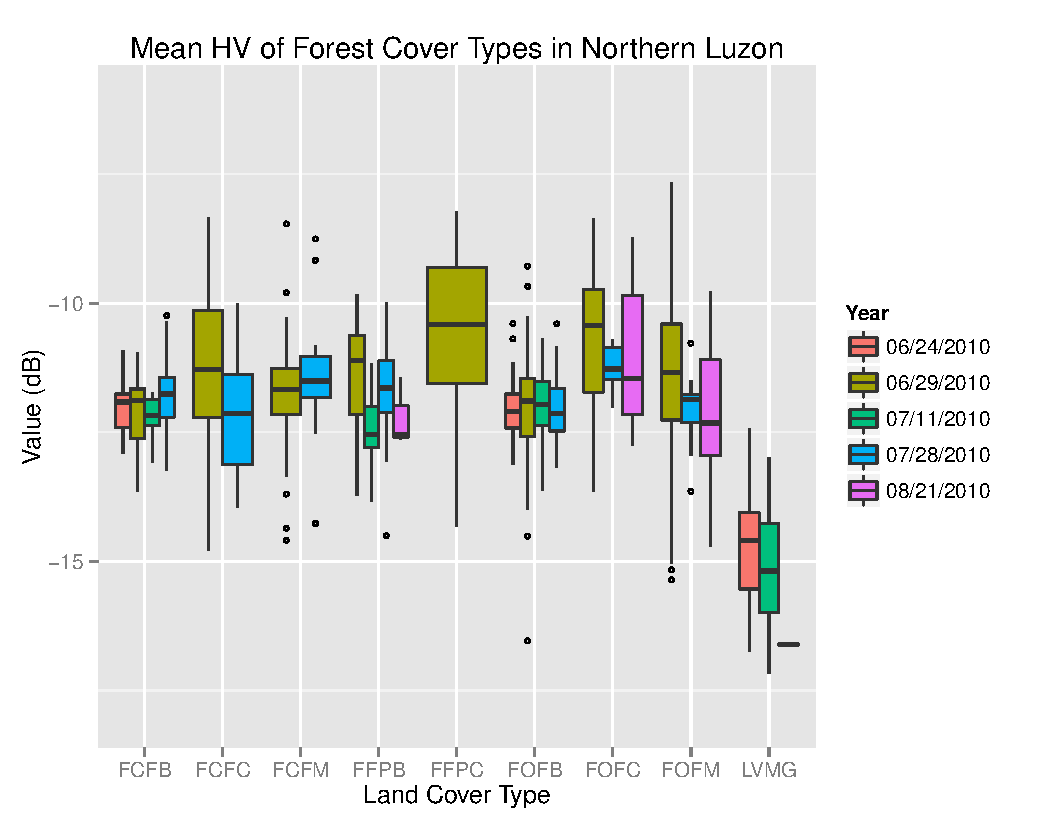
\includegraphics[width=\textwidth]{fig_boxplot-2010-mean-hv.pdf}
		\caption[Single year backscatter boxplots.]{2010 Mean HV.}
		\label{fig: result-box4.2e}
	\end{subfigure}
	\begin{subfigure}[t]{0.43\textwidth}
		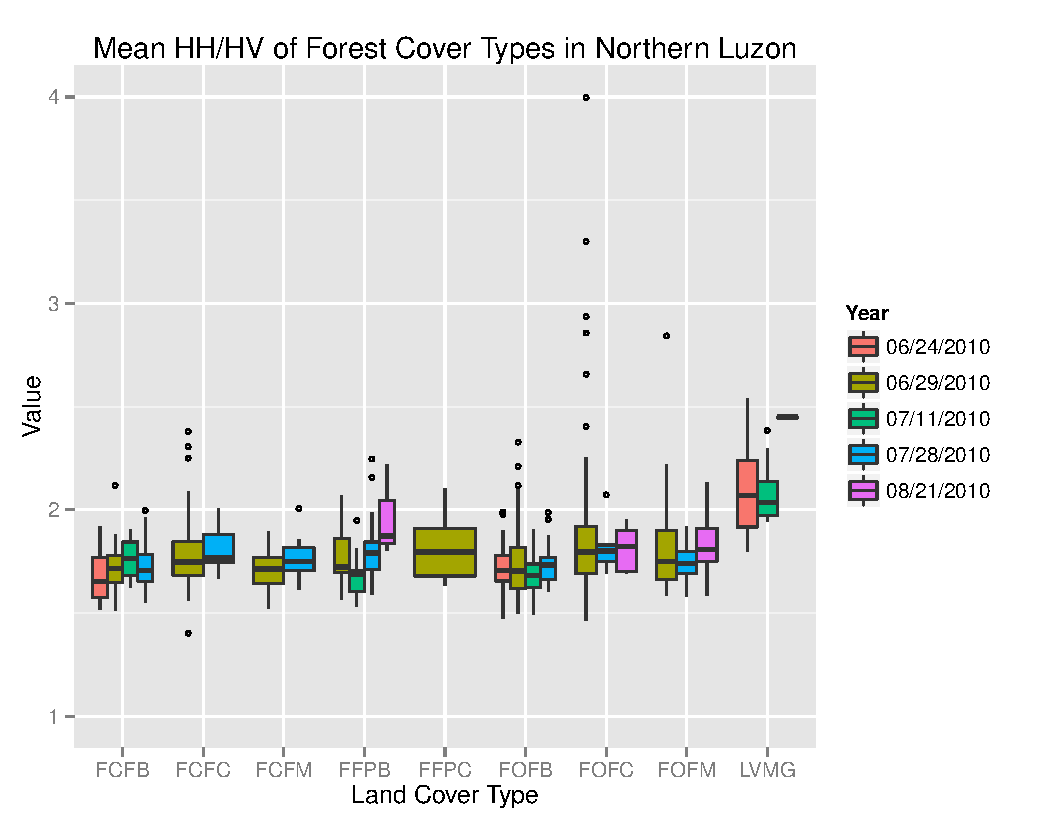
\includegraphics[width=\textwidth]{fig_boxplot-2010-mean-rat.pdf}
		\caption[Single year backscatter boxplots.]{2010 Mean HH/HV.}
		\label{fig: result-box4.2f}
	\end{subfigure}\\
	\vspace{20pt}
	\caption[Backscatter values of forest types from PALSAR data acquired in a single year at different seasons.]{Backscatter values of forest types from PALSAR data acquired in a single year at different seasons. Shown are box-whisker plots of mean backscatter values in 2009 (a-c) and 2010 (d-f).}
	\label{fig: result-box4.2}
\end{figure}
\end{landscape}

\begin{figure}[!ht] \centering
	\captionsetup[subfigure]{width=2.0in} % <-- Use this to control text which is poorly spaced under a subfigure. 
	\begin{subfigure}[t]{0.75\textwidth}
		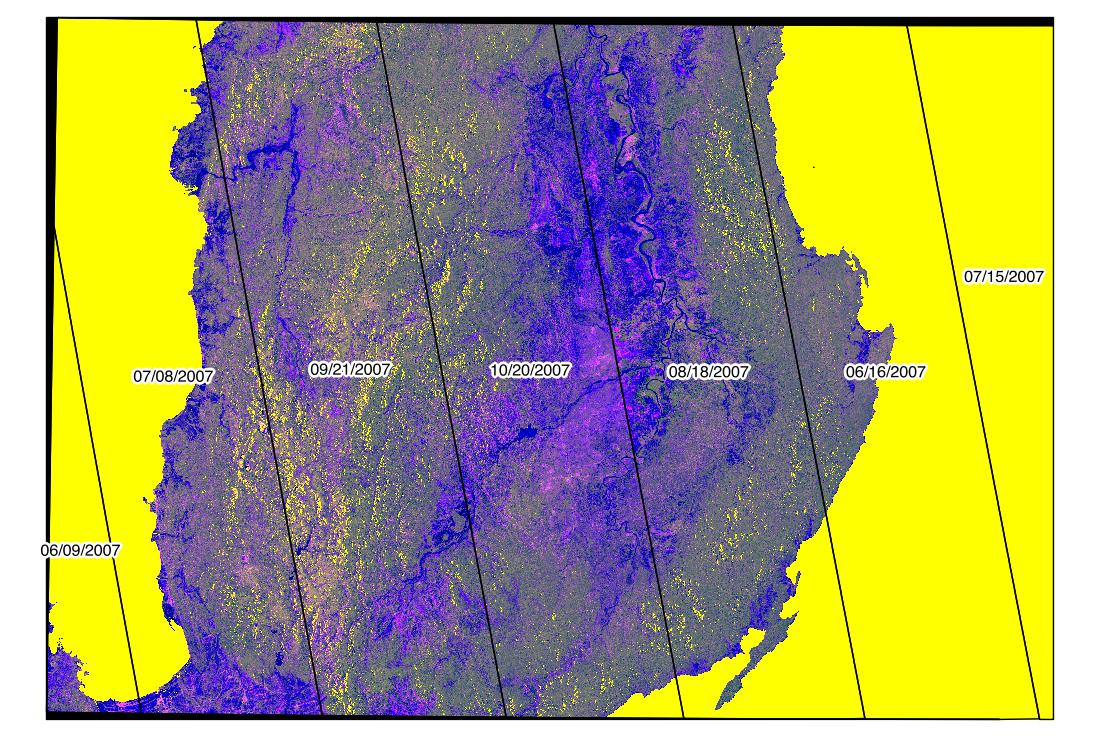
\includegraphics[width=\textwidth]{box_palsar-2007-dates.jpg}
		\caption[Box.1]{}
		\label{box: result-box4.3a}
	\end{subfigure}
	\vspace{5pt}
	\begin{subfigure}[t]{0.75\textwidth}
		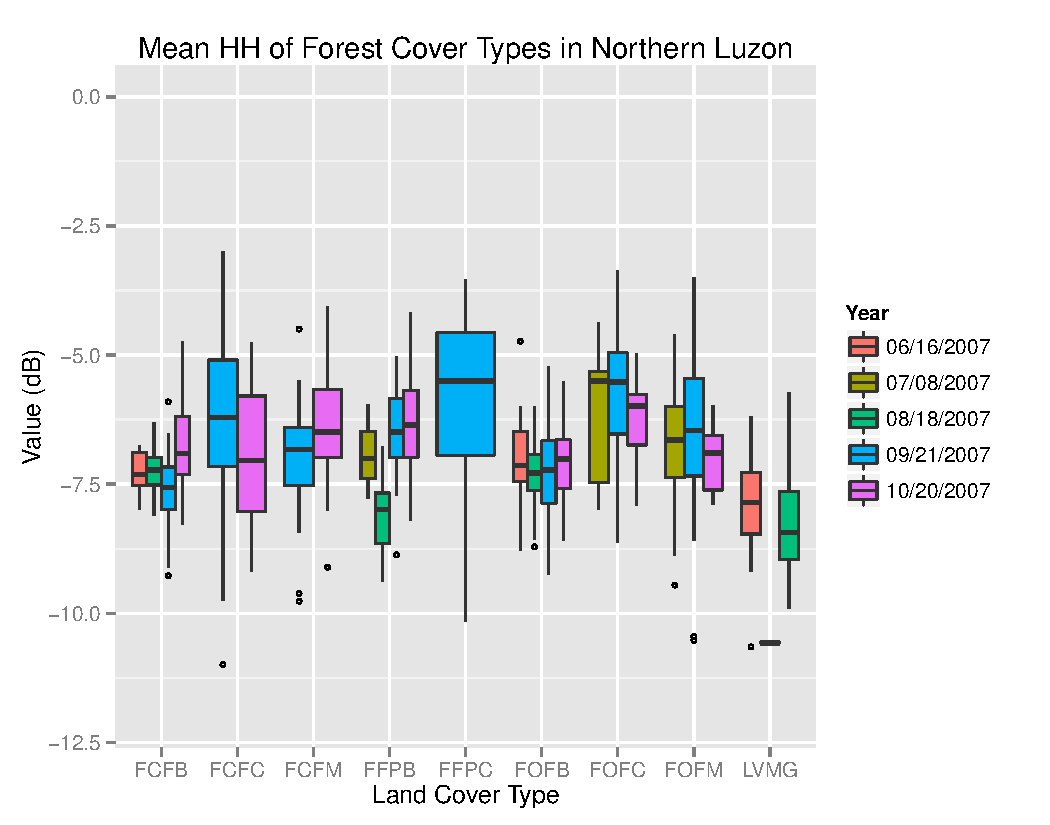
\includegraphics[width=\textwidth]{box_boxplot-2007-mean-hh.pdf}
		\caption[Box.1]{}
		\label{box: result-box4.3b}
	\end{subfigure}\\
	\caption[Box.1. The 2007 PALSAR mosaic image and the dates of acquisition of each strip/path that comprise the whole mosaic, and the distribution of mean HH backscatter for each forest cover type based on the 2007 mosaic image.]{The 2007 PALSAR mosaic image and the dates of acquisition of each strip/path that comprise the whole mosaic (a), and the distribution of mean HH backscatter for each forest cover type (b) based on the 2007 mosaic image.}
	\label{box: result-box4.3}
\end{figure}

\begin{figure}[!ht] \centering
	\captionsetup[subfigure]{width=2.0in} % <-- Use this to control text which is poorly spaced under a subfigure. 
	\begin{subfigure}[t]{0.75\textwidth}
		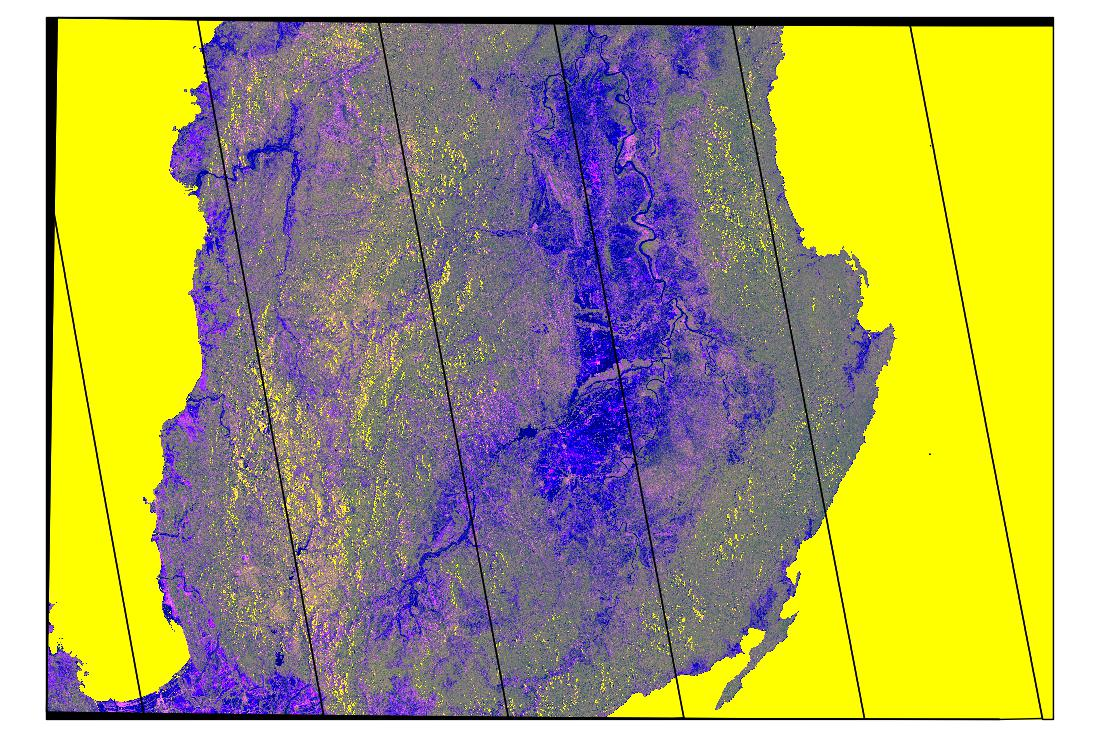
\includegraphics[width=\textwidth]{box_palsar-2010-nodates.jpg}
		\caption[Box.2]{}
		\label{box: result-box4.4a}
	\end{subfigure}
	\vspace{5pt}
	\begin{subfigure}[t]{0.75\textwidth}
		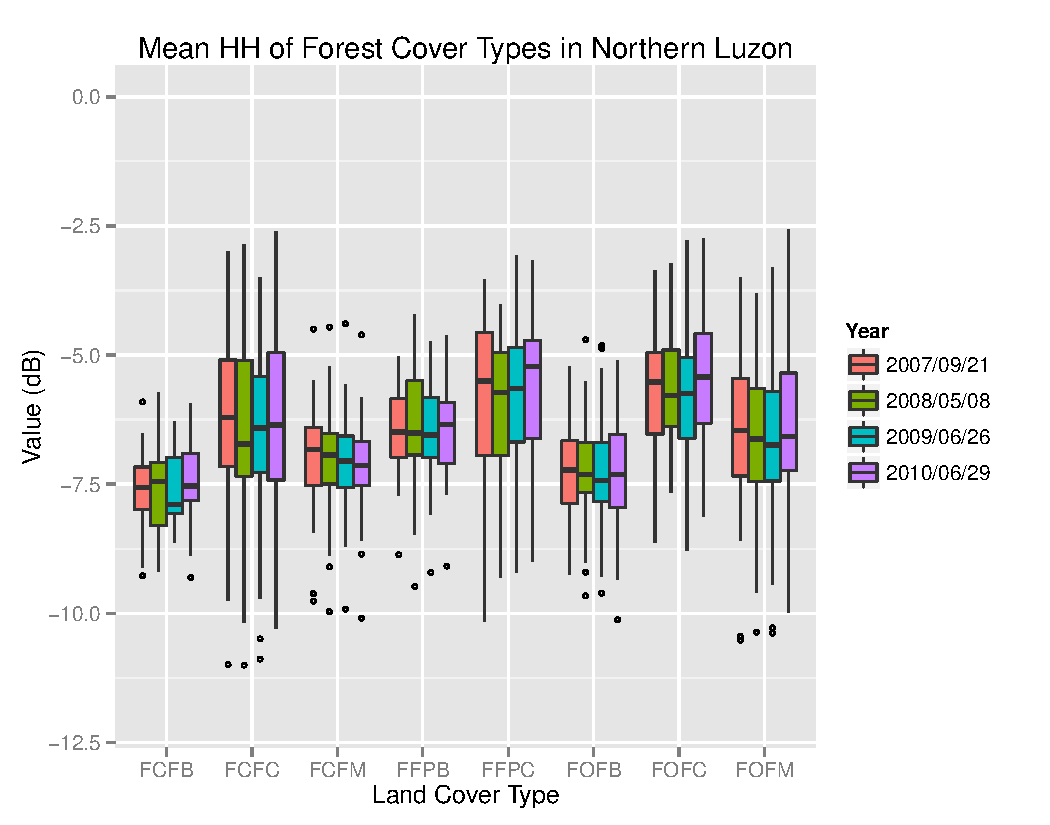
\includegraphics[width=\textwidth]{box_boxplot-strip1-mean-hh.pdf}
		\caption[Box.2]{}
		\label{box: result-box4.4b}
	\end{subfigure}\\
	\caption[Box.2. A PALSAR mosaic image highlighting the strip/path where ROIs of forest cover types were taken across four years, and the distribution of mean HH backscatter for each forest cover type along the same strip at different years.]{A PALSAR mosaic image highlighting the strip/path where ROIs of forest cover types were taken across four years (a), and the distribution of mean HH backscatter for each forest cover type (b) along the same strip at different years.}
	\label{box: result-box4.4}
\end{figure}

\begin{figure}[!ht] \centering
	\captionsetup[subfigure]{width=2.0in} % <-- Use this to control text which is poorly spaced under a subfigure. 
	\begin{subfigure}[t]{0.49\textwidth}
		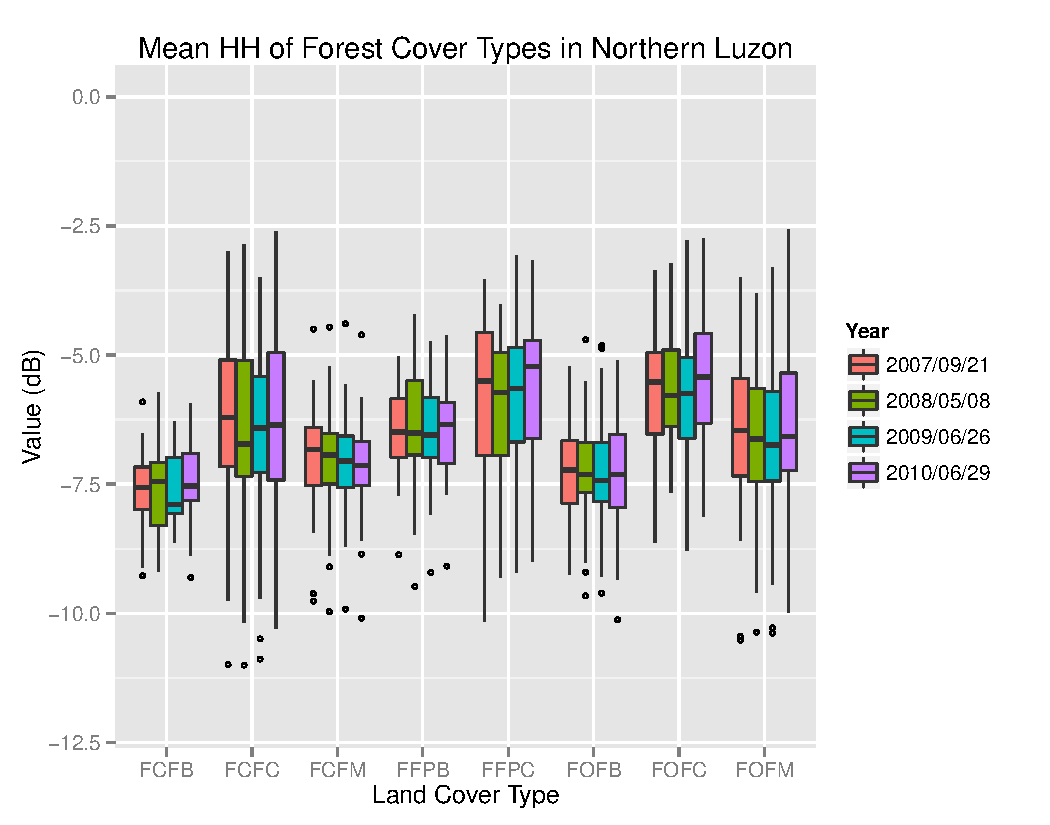
\includegraphics[width=\textwidth]{fig_boxplot-strip1-mean-hh.pdf}
		\caption[Same strip backscatter boxplots.]{Mean HH}
		\label{fig: result-fig4.5a}
	\end{subfigure}
	\begin{subfigure}[t]{0.49\textwidth}
		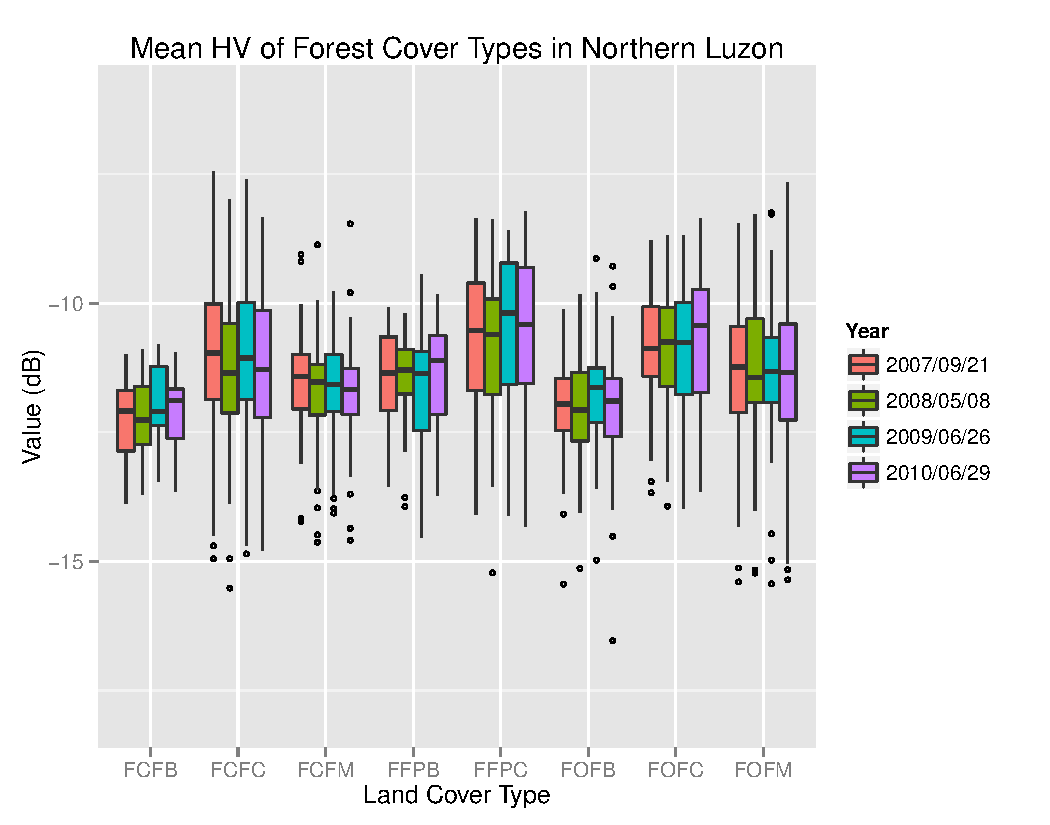
\includegraphics[width=\textwidth]{fig_boxplot-strip1-mean-hv.pdf}
		\caption[Same strip backscatter boxplots.]{Mean HV}
		\label{fig: result-fig4.5b}
	\end{subfigure}\\
	\vspace{10pt}
	\begin{subfigure}[t]{0.49\textwidth}
		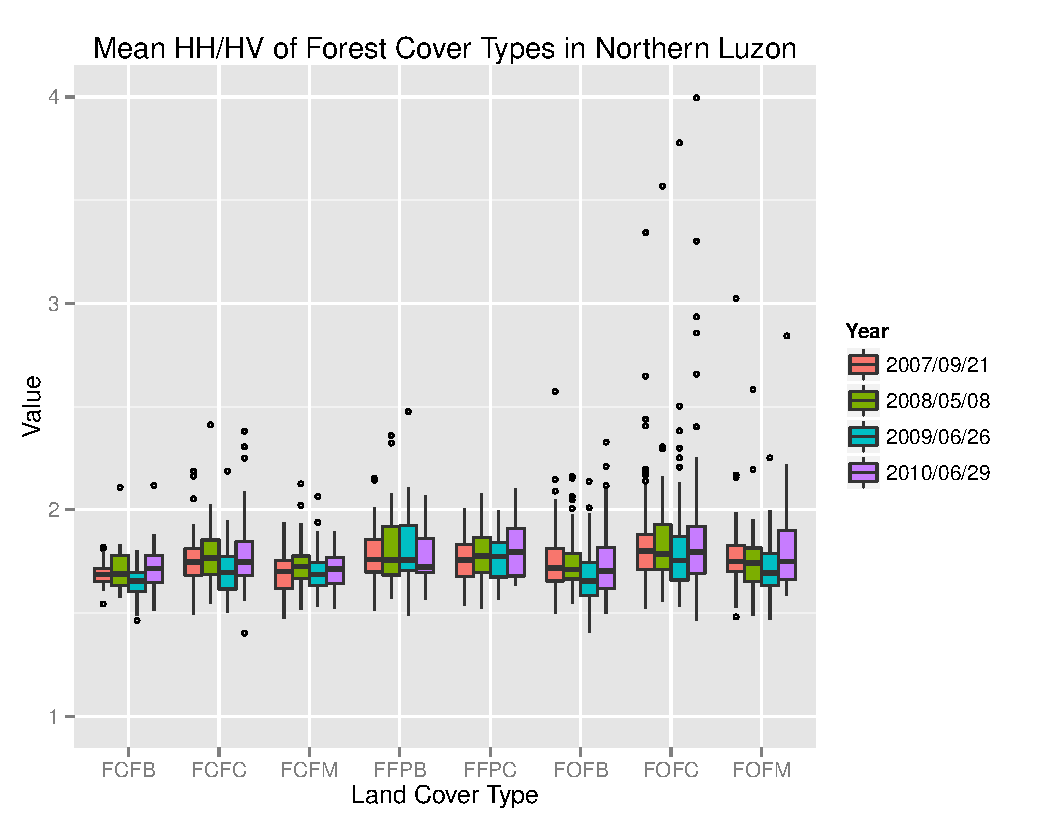
\includegraphics[width=\textwidth]{fig_boxplot-strip1-mean-rat.pdf}
		\caption[Same strip backscatter boxplots.]{Mean HH/HV}
		\label{fig: result-fig4.5c}
	\end{subfigure}
	\begin{subfigure}[t]{0.49\textwidth}
		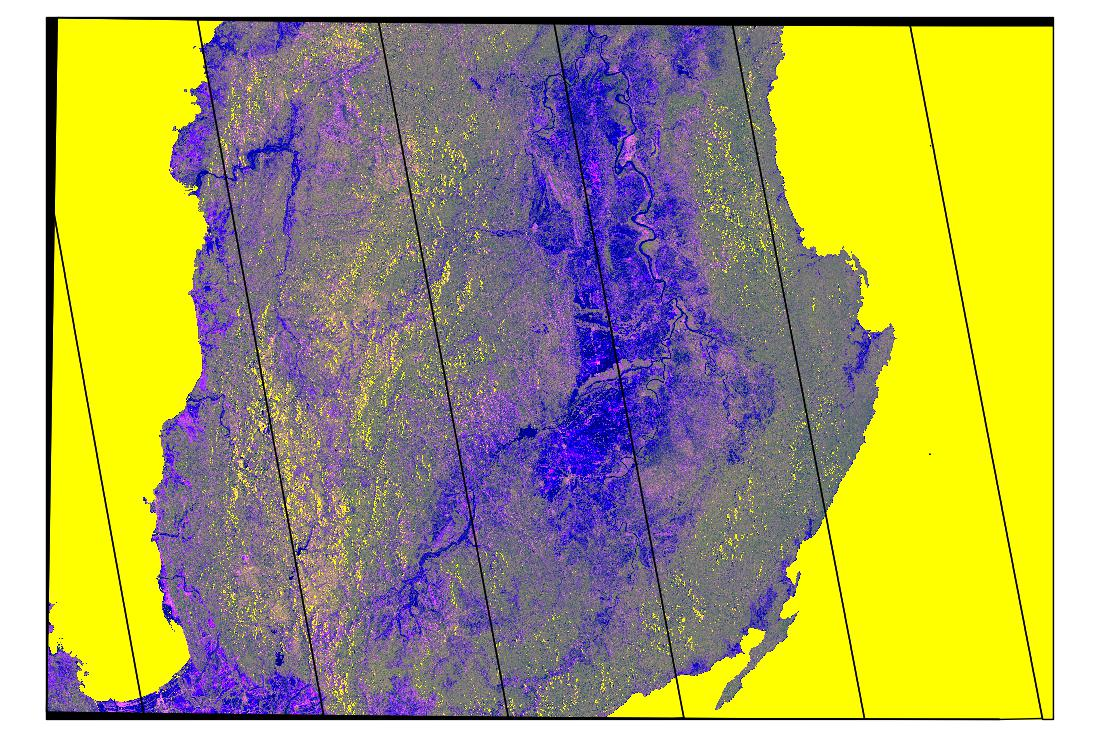
\includegraphics[width=\textwidth]{box_palsar-2010-nodates.jpg}
		\caption[Same strip backscatter boxplots.]{Strip 1}
		\label{fig: result-fig4.5d}
	\end{subfigure}
	\caption[Backscatter values of forest types from PALSAR data acquired along the same strip (Cordillera) at different years.]{Backscatter values of forest types from PALSAR data acquired along the same strip (Cordillera) at different years.}
	\label{fig: result-fig4.5}
\end{figure}

\begin{figure}[!ht] \centering
	\captionsetup[subfigure]{width=2.0in} % <-- Use this to control text which is poorly spaced under a subfigure. 
	\begin{subfigure}[t]{0.49\textwidth}
		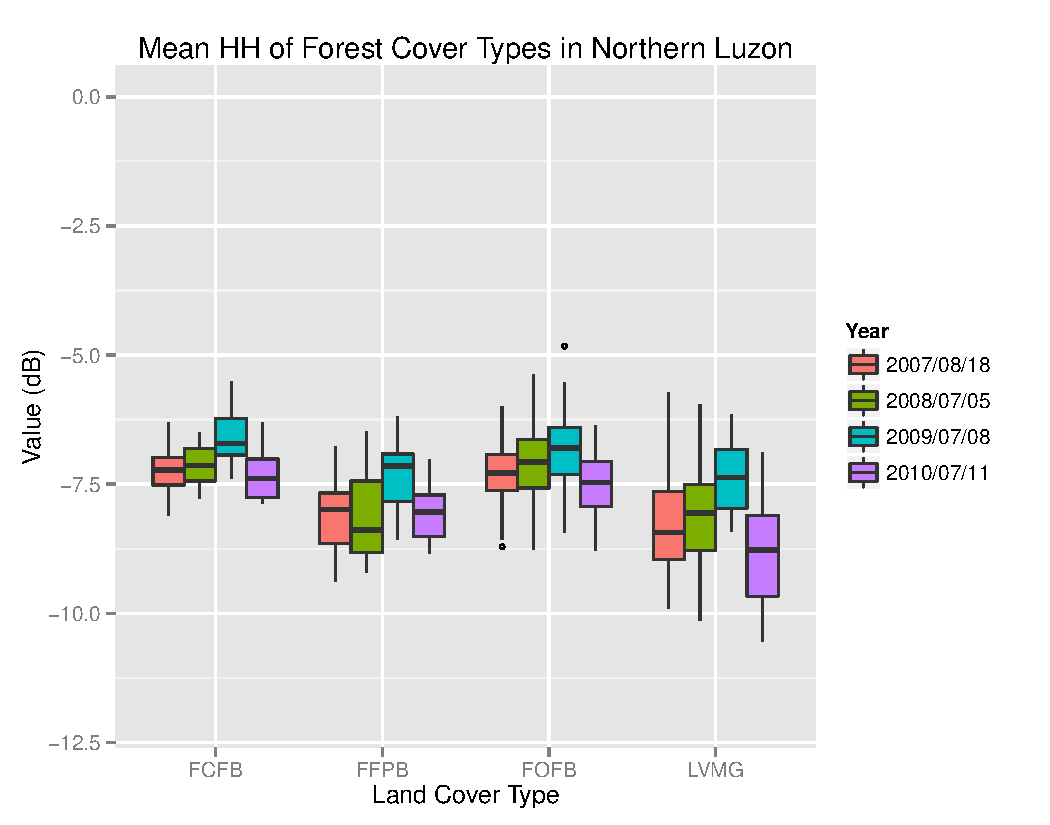
\includegraphics[width=\textwidth]{fig_boxplot-strip2-mean-hh.pdf}
		\caption[Same strip backscatter boxplots.]{Mean HH}
		\label{fig: result-fig4.6a}
	\end{subfigure}
	\begin{subfigure}[t]{0.49\textwidth}
		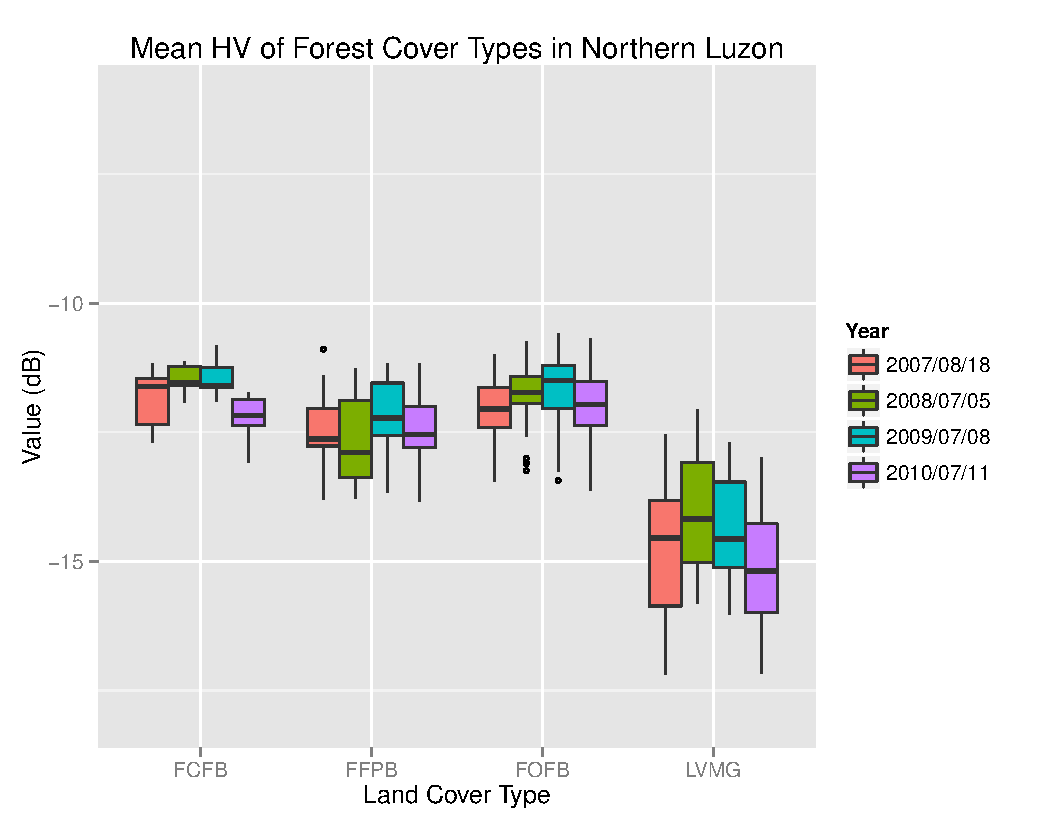
\includegraphics[width=\textwidth]{fig_boxplot-strip2-mean-hv.pdf}
		\caption[Same strip backscatter boxplots.]{Mean HV}
		\label{fig: result-fig4.6b}
	\end{subfigure}\\
	\vspace{10pt}
	\begin{subfigure}[t]{0.49\textwidth}
		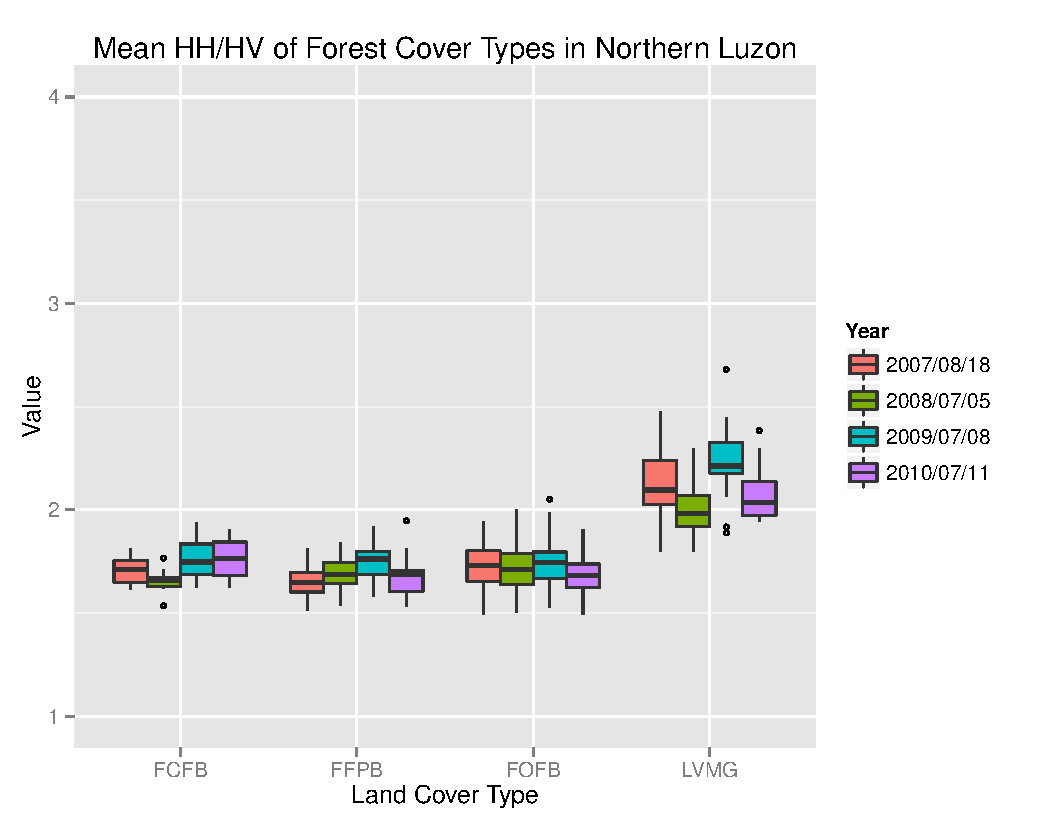
\includegraphics[width=\textwidth]{fig_boxplot-strip2-mean-rat.pdf}
		\caption[Same strip backscatter boxplots.]{Mean HH/HV}
		\label{fig: result-fig4.6c}
	\end{subfigure}
	\begin{subfigure}[t]{0.49\textwidth}
		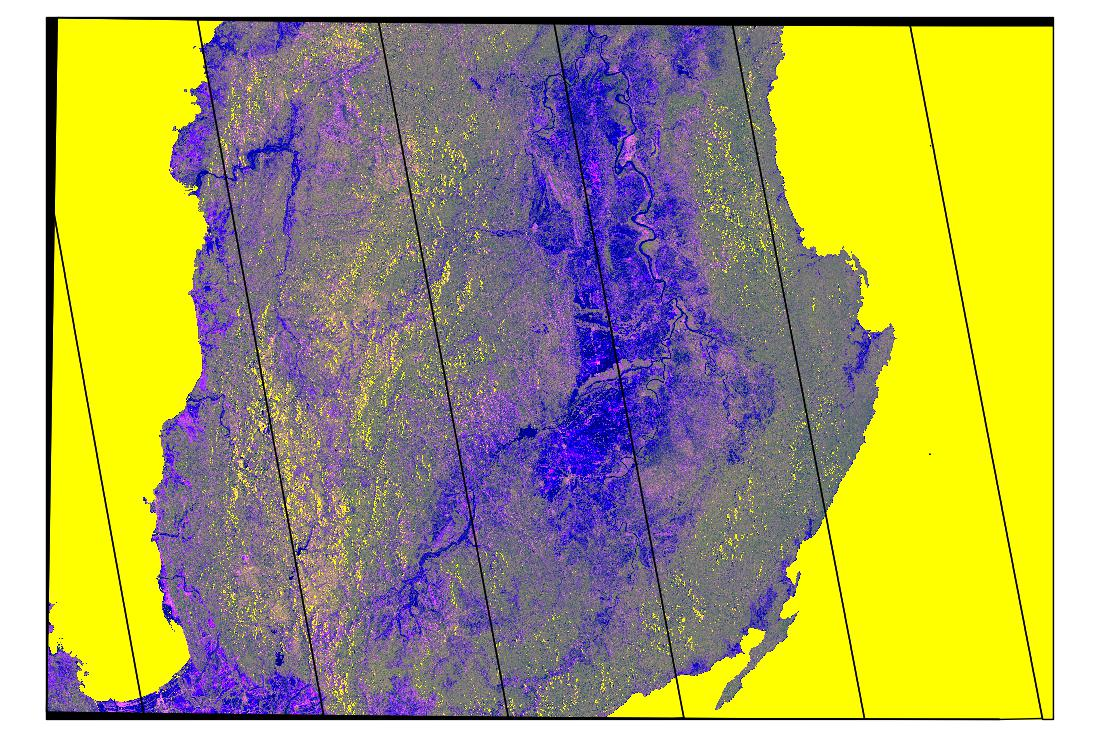
\includegraphics[width=\textwidth]{box_palsar-2010-nodates.jpg}
		\caption[Same strip backscatter boxplots.]{Strip 2}
		\label{fig: result-fig4.6d}
	\end{subfigure}
	\caption[Backscatter values of forest types from PALSAR data acquired along the same strip (Sierra Madre) at different years.]{Backscatter values of forest types from PALSAR data acquired along the same strip (Sierra Madre) at different years.}
	\label{fig: result-fig4.6}
\end{figure}

\section{Consistency of forest classification hierarchy}
\label{sec: result-hierarchy-consistency}

\begin{figure}
	\centering
	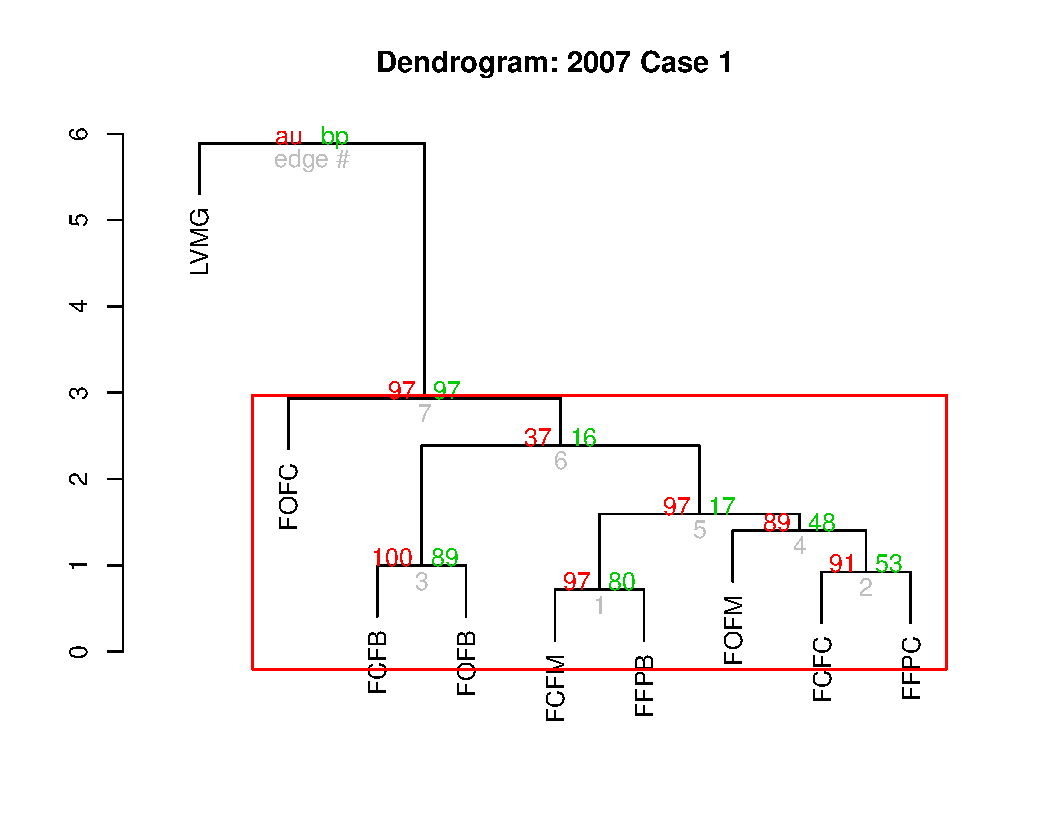
\includegraphics[width=1.0\textwidth]{box_dendrogram-2007-case1.pdf}
	\caption[Box 3. Example dendrogram result from the hierarchical clustering of forest cover types using polarimetric feature attributes (Case 1) from the 2007 PALSAR mosaic image.]{Example dendrogram result from the hierarchical clustering of forest cover types using polarimetric feature attributes (Case 1) from the 2007 PALSAR mosaic image.}
	\label{fig: result-fig4.7}
\end{figure}

A total of 16 dendrograms were produced from the hierarchical cluster analysis consisting of four dendrograms for each case (covering four years in each case). Each case represents a combination of object-level feature attributes (Table \ref{tab: method-table3.3}), particularly: Case 1 using Polarisation feature attributes; Case 2 using Polarisation and Topographic; Case 3 using Polarisation and Texture; and Case 4 using all feature attributes (Polarisation, Topographic, Texture).

As an example, the figure in Fig. \ref{fig: result-fig4.7}, which was taken from Fig. \ref{fig: result-fig4.8}, shows the dendrogram resulting from the hierarchical clustering of forest cover types using polarimetric feature attributes from the 2007 PALSAR mosaic image. The dendrogram shows which forest types are similar or dissimilar from other types. The y-axis indicates the computed distance between clusters using an average linkage algorithm in determining which clusters are similar. Within the tree structure, the edge numbers denoted in grey colour indicate the sequence of the grouping of nodes into similar clusters given that an agglomerative hierarchical clustering technique was used, and the red value indicates the AU p-value, of which values $\geq$ 0.95 represents consistent grouping. The red box indicates which clusters or groups of clusters have $\geq$ 0.95 AU p-values, and hence have consistent groupings.

In this dendrogram, Cluster \#1 showed that closed canopy mixed forest (FCFM) and broadleaved forest plantation (FFPB) were similar with a 97 AU p-value. Next, Cluster \#2 showed closed canopy coniferous forest (FCFC) and coniferous forest plantation (FFPC) were similar with 91 AU p-value. Cluster \#3 showed closed canopy broadleaved forest (FCFB) and open canopy broadleaved forest (FOFB) were similar with 100 AU p-value, suggesting that closed and open canopy broadleaved forests were similar in this case using polarimetric attributes. Cluster \#4 showed Cluster \#2 being grouped together with open canopy mixed forest (FOFM) at 89 AU p-value, and subsequently grouped with Cluster \#1 as Cluster \#5 at 97 AU p-value. All the forest types in Cluster \#5 were subsequently grouped together with Cluster \#3 at only 37 AU p-value. Then, all the forest types in Cluster \#6 were grouped with open canopy coniferous forest (FOFC) as Cluster \#7 with 97 AU p-value. Finally, Cluster \#8 showed mangrove forest (LVMG) grouped with all other forest types in Cluster \#7, suggesting that mangroves had greatest dissimilarity from the rest of the forest types.\\

\begin{spacing}{1.0}
\begin{longtable}[h!]{ p{2.5cm} p{2.6cm} p{2.8cm} p{2.6cm} p{2.5cm} }

    \caption[Baker's Gamma Indices ($\beta$ coefficients) per case for each pair of years.]{Baker's Gamma Indices ($\beta$ coefficients) per case for each pair of years.}
    \label{tab: result-table4.1}\\
    
    	\toprule
    	Years & {} & Baker's Gamma & ($\beta$ Coefficient) & {}\\
    	\cmidrule{2-5}
    	{} & Case 1 & Case 2 & Case 3 & Case 4\\
    	\midrule
    	\endhead
    	
		2007-2008 & 0.8966454 & 0.9896552 & 0.8786650 & 0.8797485\\
		2007-2009 & 0.8527756 & 0.5834679 & 0.8078116 & 0.8393977\\
		2007-2010 & 0.8849630 & 0.9634359 & 0.8301529 & 0.8250326\\
		2008-2009 & 0.8853727 & 0.6208636 & 0.8750541 & 0.8914641\\
		2008-2010 & 0.9899121 & 0.9706925 & 0.8943540 & 0.8950236\\
		2009-2010 & 0.8858105 & 0.6269121 & 0.9539378 & 0.8526550\\
				
		\bottomrule \\
    
\end{longtable}
\end{spacing}

For Case 1, the dendrograms showed the clustering of forest types using only polarimetric feature attributes (Fig. \ref{fig: result-fig4.8}). Except for 2009, AU p-values for the other years were all greater than 0.95 indicating reliable clustering results, specifically for 8 of 9 forest types. Mangrove forest (LVMG) and open coniferous forest (FOFC) appeared as distinct clusters across all years. The $\beta$ coefficients were all high (\textgreater0.85), which indicate relatively similar clusters or dendrogram structure across all four years (Table \ref{tab: result-table4.1}).

For Case 2, the dendrograms showed the clustering of forest types using polarimetric and topographic feature attributes (Fig. \ref{fig: result-fig4.9}). Both 2007 and 2008 exhibited AU p-values above 0.95. For 2009, only two clusters exhibited above 0.95 AU p-values, while 2010 did not at all. Mangrove forest (LVMG) also appeared as distinct clusters across all years. The $\beta$ coefficients were high (\textgreater0.96) for pairwise combinations that do not include 2009, of which values were average (range from 0.58 to 0.63) (Table \ref{tab: result-table4.1}). Interestingly, except 2009, broadleaved forest types (i.e., closed, open, and plantation) and both coniferous and mixed forest types (i.e., closed, open, and plantation) branched into separate clusters, suggesting the distinction of these general forest types.

For Case 3, the dendrograms showed the clustering of forest types using polarimetric and texture feature attributes (Fig. \ref{fig: result-fig4.10}). All years exhibited stable clustering results for 8 of 9 forest types, except 2009 with only 7 of 9 forest types. Mangrove forest (LVMG) and coniferous forest plantations (FFPC) appeared as distinct clusters across all years. The $\beta$  coefficients were all high (\textgreater0.80), which indicate relatively similar clusters or dendrogram structures across all four years (Table \ref{tab: result-table4.1}).

For Case 4, the dendrograms showed the clustering of forest types using all feature attributes, including polarimetric, topographic, and texture (Fig. \ref{fig: result-fig4.11}). The AU p-values consisting of majority of forest types were above 0.95 for 2007, 2008, and 2009. For 2010, only one terminal cluster exhibited above 0.95 AU p-value. Similar to Case 3, mangrove forest (LVMG) and coniferous forest plantations (FFPC) appeared as distinct clusters across all years. The $\beta$ coefficients were all high (\textgreater0.82), which indicate relatively similar clusters or dendrogram structure across all four years (Table \ref{tab: result-table4.1}).\\

\begin{spacing}{1.0}
\begin{longtable}[h!]{ p{1cm} p{1.4cm} p{1.4cm} p{1.4cm} p{1.4cm} p{1.4cm} p{1.4cm} p{1.4cm} p{0.9cm} }

    \caption[Summary of Baker's Gamma Indices ($\beta$ coefficients) for pairwise comparison of dendrograms across all cases.]{Summary of Baker's Gamma Indices ($\beta$ coefficients) for pairwise comparison of dendrograms across all cases.}
    \label{tab: result-table4.2}\\
    
    	\toprule
    	Case & {} 07-08 & 07-09 & 07-10 & 08-09 & 08-10 & 09-10 & Total & Rank\\
    	\midrule
    	\endhead
    	
		1 & 0.89664 & 0.85277 & 0.88496 & 0.88537 & 0.98991 & 0.88581 & 5.39547 & 1\\
		2 & 0.98965 & 0.58346 & 0.96343 & 0.62086 & 0.97069 & 0.62691 & 4.75502 & 4\\
		3 & 0.87866 & 0.80781 & 0.83015 & 0.87505 & 0.89435 & 0.95393 & 5.23997 & 2\\
		4 & 0.87974 & 0.83939 & 0.82503 & 0.89146 & 0.89502 & 0.85265 & 5.18332 & 3\\
		\cmidrule{1-9}
		Total & 3.64471 & 3.08345 & 3.50358 & 3.27275 & 3.74998 & 3.31931 & 3.42896 & {}\\
				
		\bottomrule \\
    
\end{longtable}
\end{spacing}

The Baker's Gamma Indices for pairwise comparison of dendrograms were tabulated across all cases to assess the effect of topographic and texture feature attributes, in addition to polarisation, on the consistency of the hierarchies between dendrograms (Table \ref{tab: result-table4.2}). Pairwise dendrogram comparisons involving the 2009 ALOS/PALSAR image showed lower consistencies as shown by vertical sum of coefficients for each pairwise comparison.

High Baker's Gamma Index coefficients (i.e., values close to 1) resulting from pairwise comparisons of dendrograms between acquisition years indicated that the hierarchical clustering of forest types were similar and consistent across years, and reinforced the temporal consistency of the ALOS/PALSAR mosaic data acquired in different years. Ranking showed that polarimetric variables (Case 1) had the highest consistencies between pairwise dendrogram comparisons. This suggests that polarimetric data by itself is temporally consistent across different acquisition years, and the forest classification hierarchy is also similarly consistent across different acquisition years. The inclusion of other feature attributes slightly lowers the consistency in both aspects. Nevertheless, nominal values of Baker’s Gamma Index coefficients were still high, suggesting that the inclusion of topographic or texture variables or both only marginally decreases the temporal consistency of ALOS/PALSAR mosaics and hierarchical consistency of the forest type classification.

\begin{figure}[!ht] \centering
	\captionsetup[subfigure]{width=2.0in} % <-- Use this to control text which is poorly spaced under a subfigure. 
	\begin{subfigure}[t]{0.49\textwidth}
		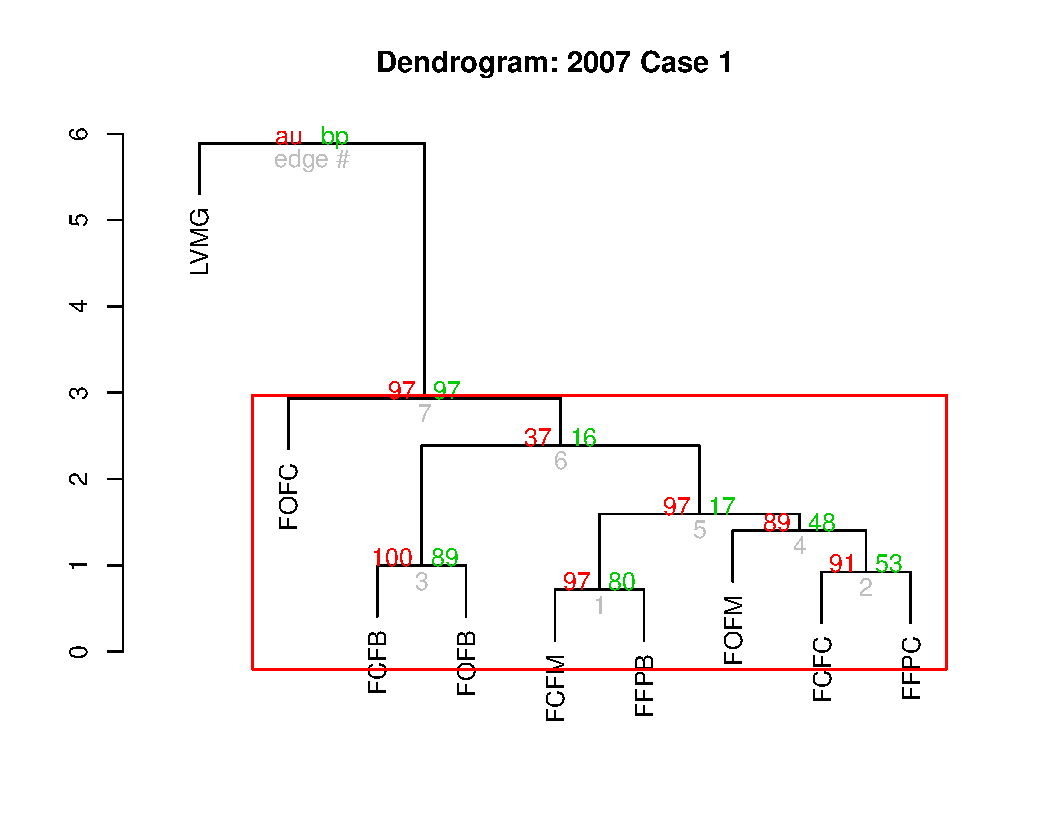
\includegraphics[width=\textwidth]{fig_dendrogram-2007-case1.pdf}
		\caption[Case 1 cluster dendrograms.]{2007 Case 1}
		\label{fig: result-fig4.8a}
	\end{subfigure}
	\begin{subfigure}[t]{0.49\textwidth}
		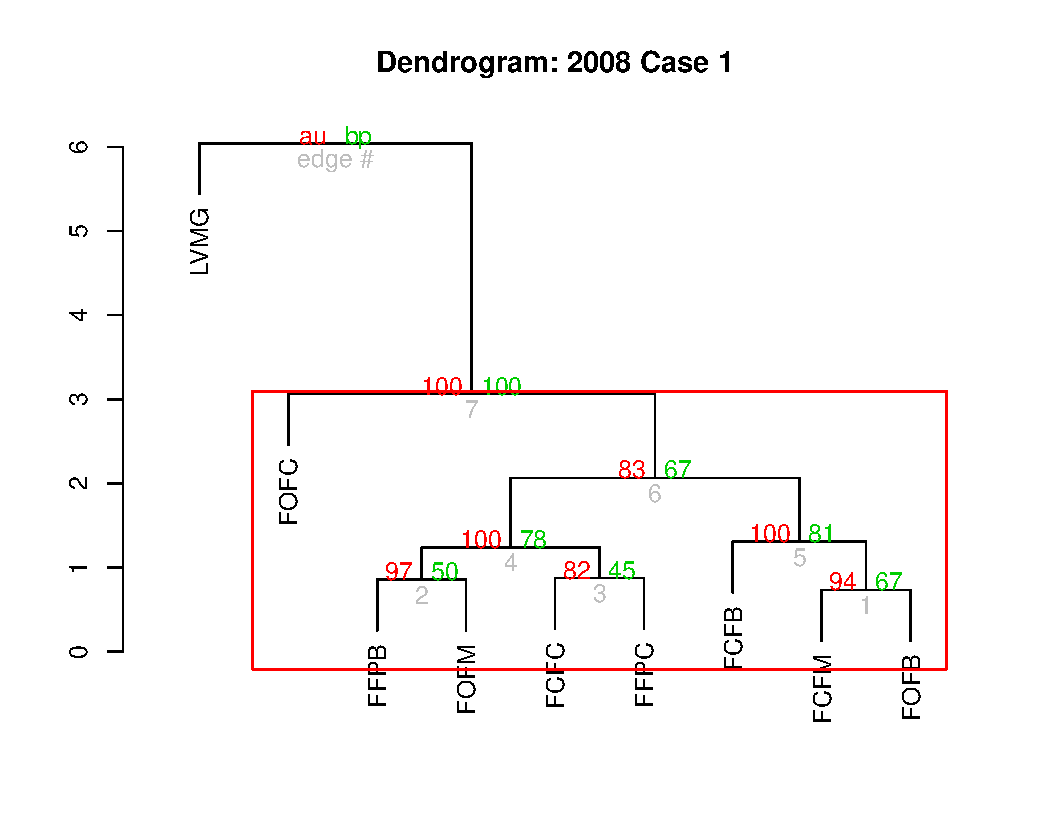
\includegraphics[width=\textwidth]{fig_dendrogram-2008-case1.pdf}
		\caption[Case 1 cluster dendrograms.]{2008 Case 1}
		\label{fig: result-fig4.8b}
	\end{subfigure}\\
	\vspace{15pt}
	\begin{subfigure}[t]{0.49\textwidth}
		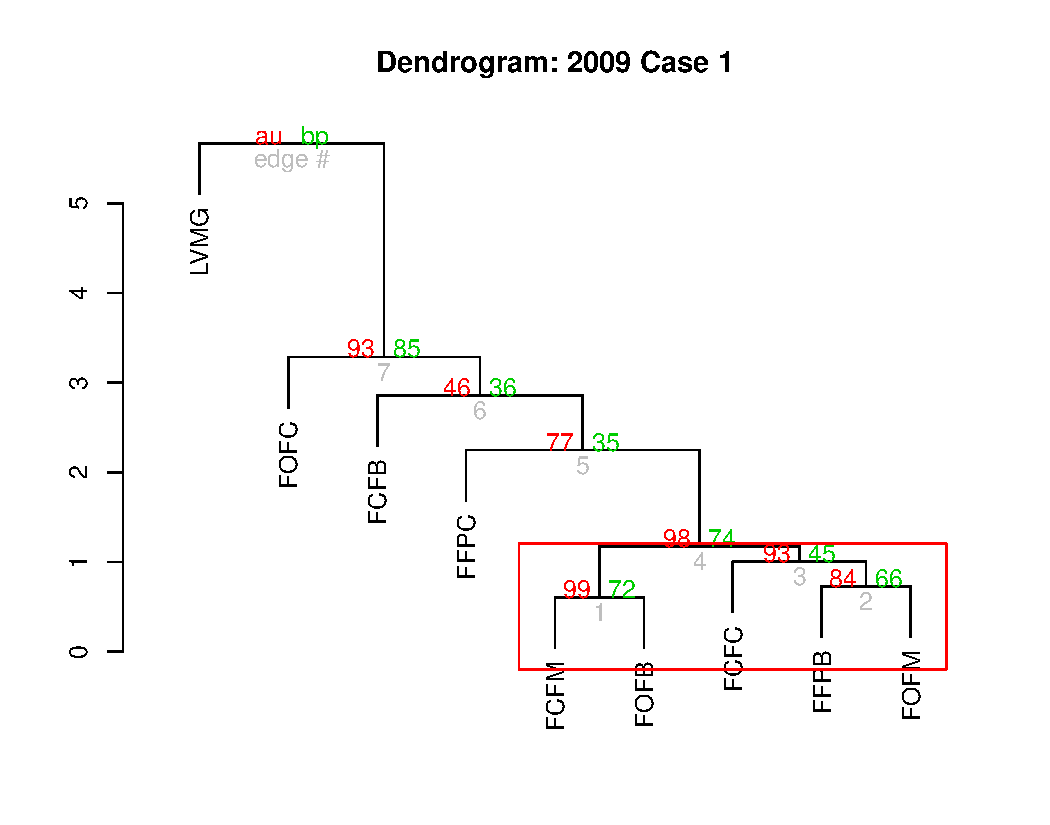
\includegraphics[width=\textwidth]{fig_dendrogram-2009-case1.pdf}
		\caption[Case 1 cluster dendrograms.]{2009 Case 1}
		\label{fig: result-fig4.8c}
	\end{subfigure}
	\begin{subfigure}[t]{0.49\textwidth}
		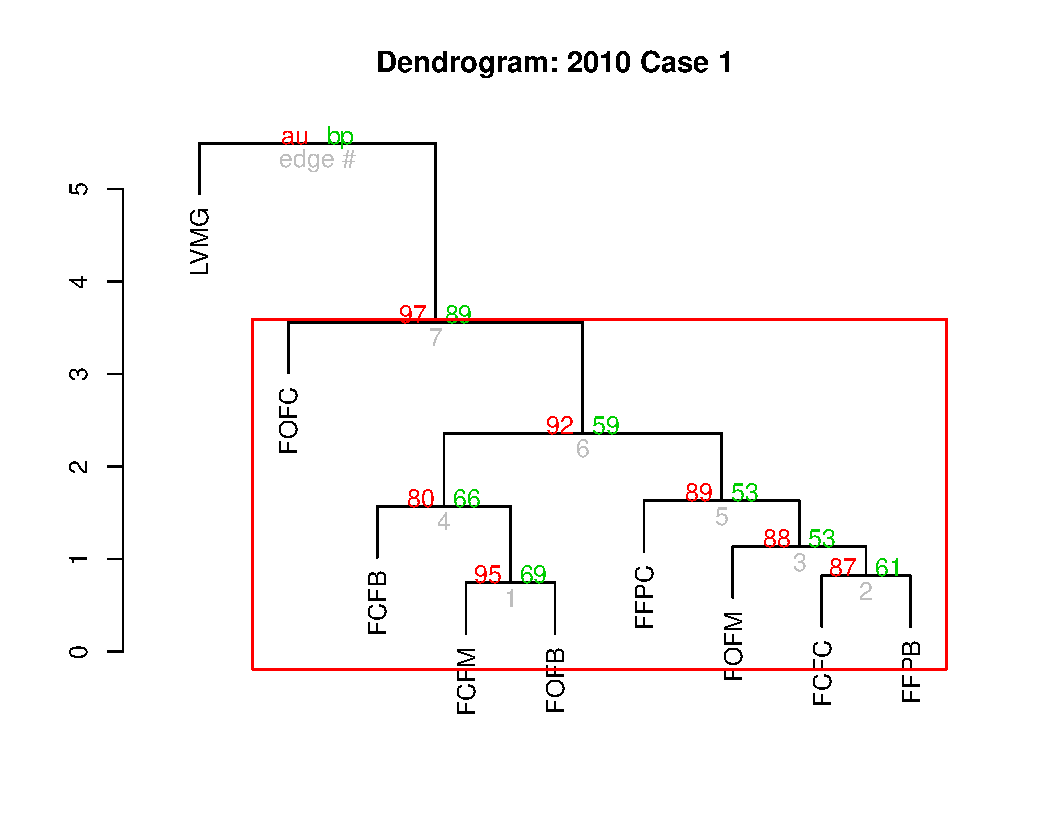
\includegraphics[width=\textwidth]{fig_dendrogram-2010-case1.pdf}
		\caption[Case 1 cluster dendrograms.]{2010 Case 1}
		\label{fig: result-fig4.8d}
	\end{subfigure}
	\vspace{5pt}
	\caption[Dendrograms from cluster analysis using Case 1.]{Dendrograms from cluster analysis using Case 1. Red boxes AU p-value $\geq$ 0.95.}
	\label{fig: result-fig4.8}
\end{figure}

\begin{figure}[!ht] \centering
	\captionsetup[subfigure]{width=2.0in} % <-- Use this to control text which is poorly spaced under a subfigure. 
	\begin{subfigure}[t]{0.49\textwidth}
		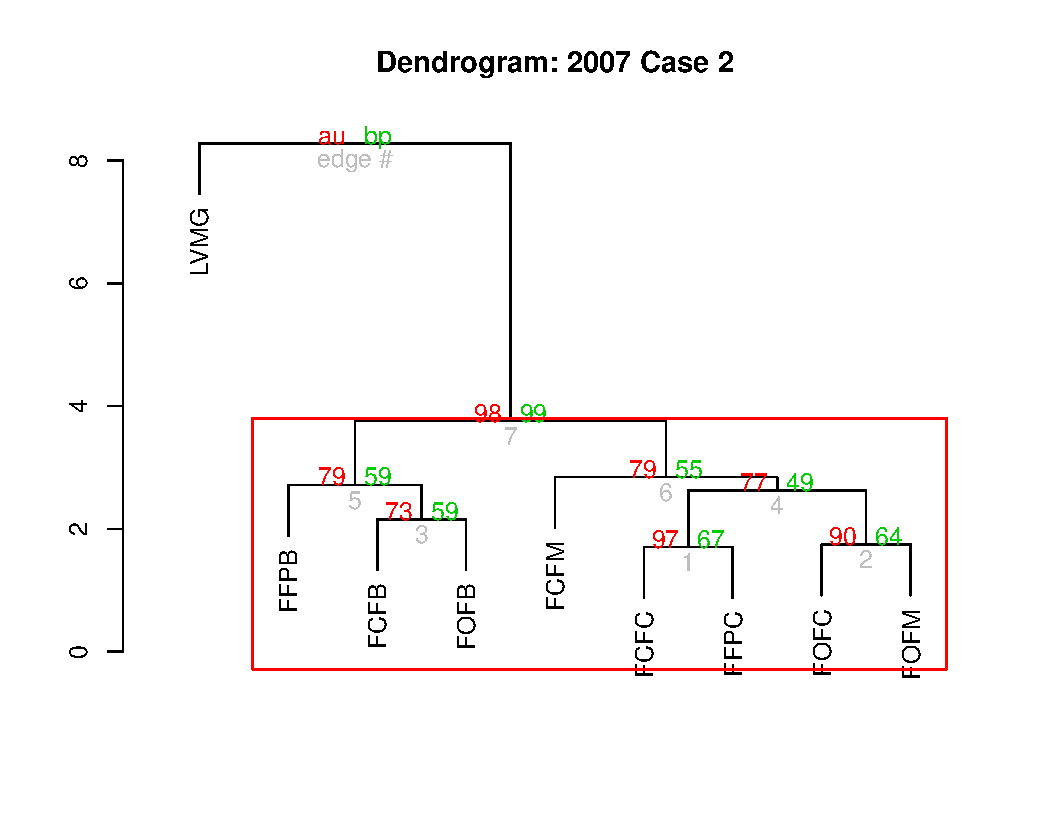
\includegraphics[width=\textwidth]{fig_dendrogram-2007-case2.pdf}
		\caption[Case 2 cluster dendrograms.]{2007 Case 2}
		\label{fig: result-fig4.9a}
	\end{subfigure}
	\begin{subfigure}[t]{0.49\textwidth}
		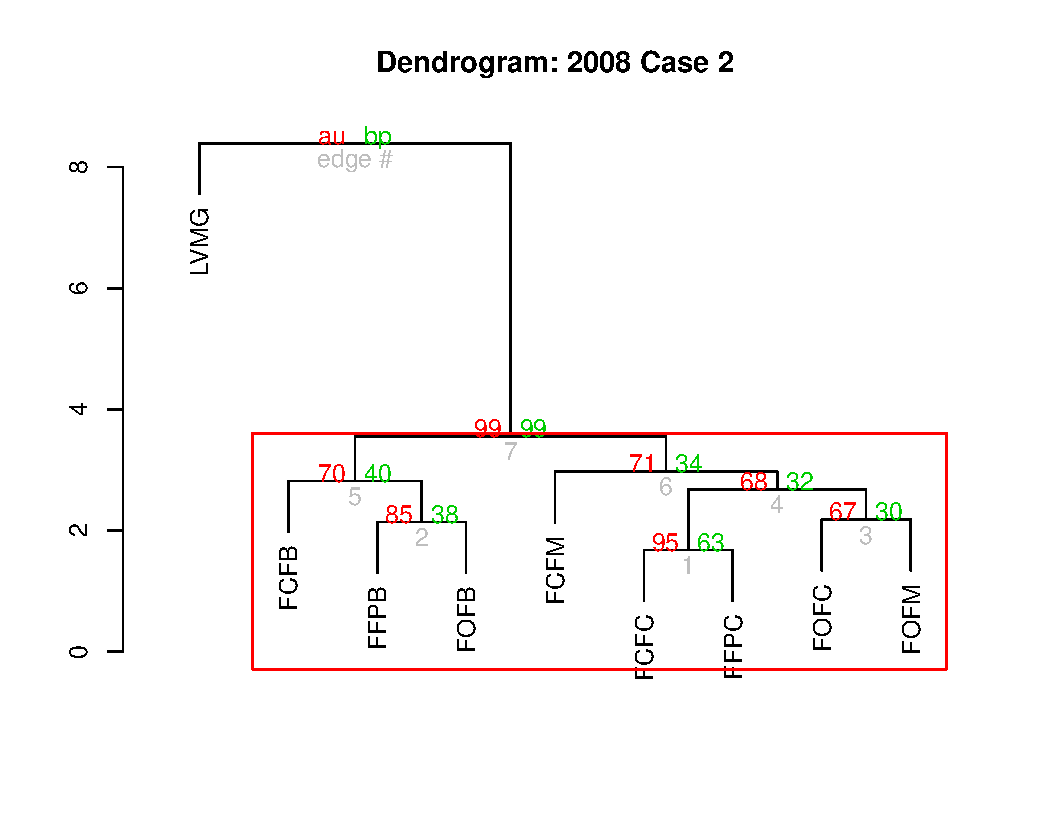
\includegraphics[width=\textwidth]{fig_dendrogram-2008-case2.pdf}
		\caption[Case 2 cluster dendrograms.]{2008 Case 2}
		\label{fig: result-fig4.9b}
	\end{subfigure}\\
	\vspace{15pt}
	\begin{subfigure}[t]{0.49\textwidth}
		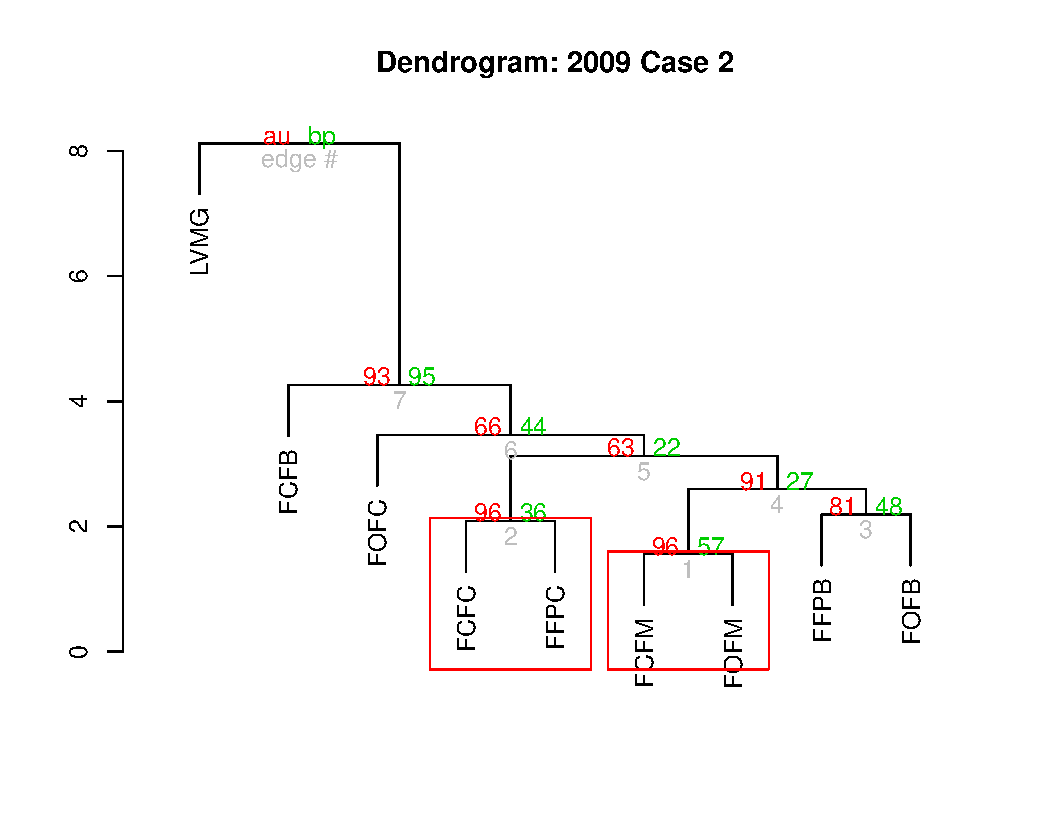
\includegraphics[width=\textwidth]{fig_dendrogram-2009-case2.pdf}
		\caption[Case 2 cluster dendrograms.]{2009 Case 2}
		\label{fig: result-fig4.9c}
	\end{subfigure}
	\begin{subfigure}[t]{0.49\textwidth}
		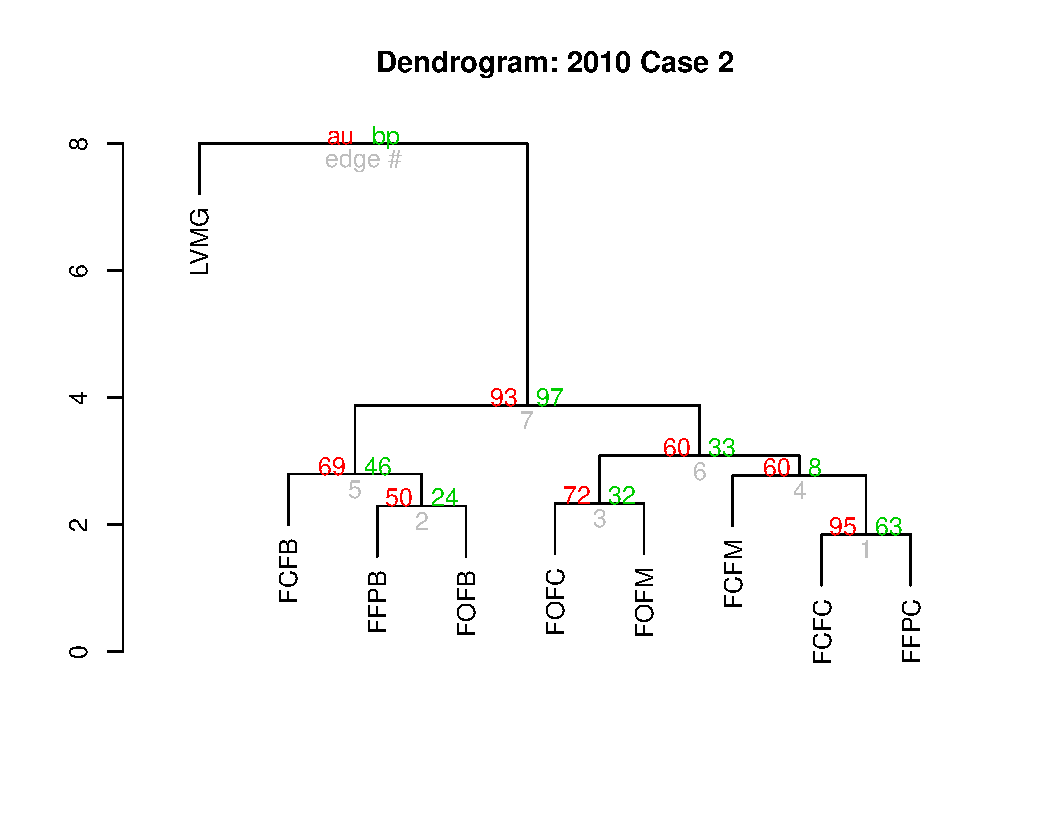
\includegraphics[width=\textwidth]{fig_dendrogram-2010-case2.pdf}
		\caption[Case 2 cluster dendrograms.]{2010 Case 2}
		\label{fig: result-fig4.9d}
	\end{subfigure}
	\vspace{5pt}
	\caption[Dendrograms from cluster analysis using Case 2.]{Dendrograms from cluster analysis using Case 2. Red boxes AU p-value $\geq$ 0.95.}
	\label{fig: result-fig4.9}
\end{figure}

\begin{figure}[!ht] \centering
	\captionsetup[subfigure]{width=2.0in} % <-- Use this to control text which is poorly spaced under a subfigure. 
	\begin{subfigure}[t]{0.49\textwidth}
		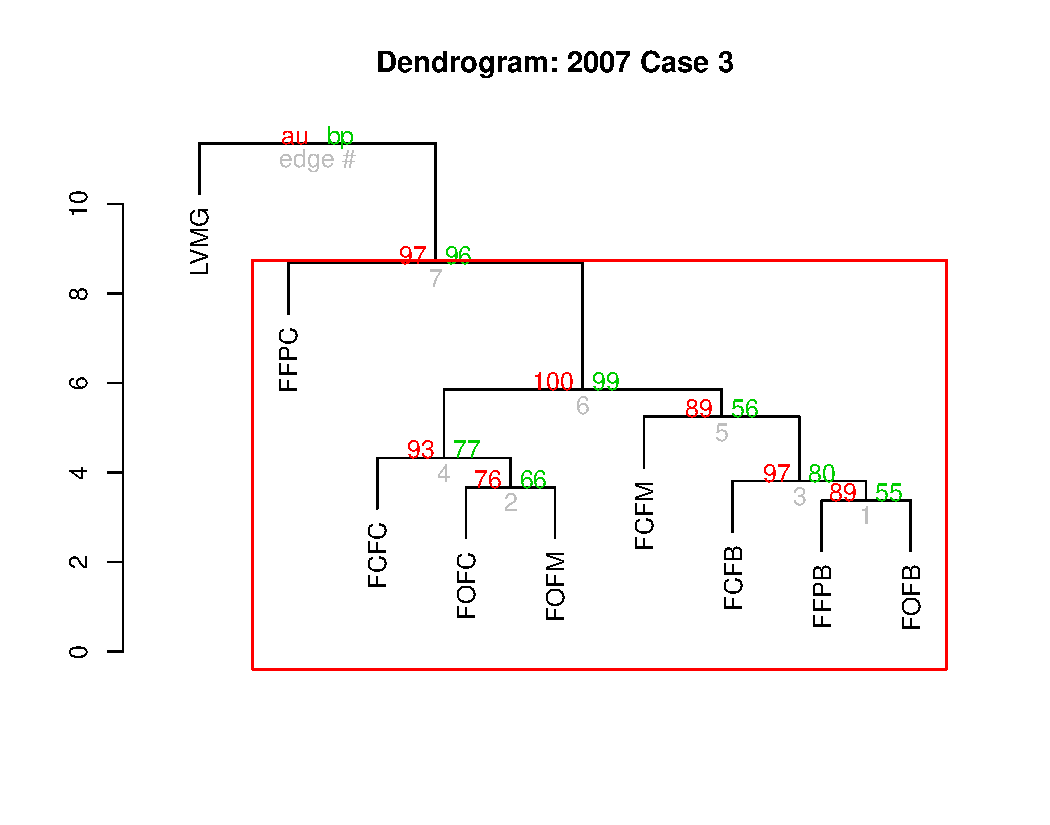
\includegraphics[width=\textwidth]{fig_dendrogram-2007-case3.pdf}
		\caption[Case 3 cluster dendrograms.]{2007 Case 3}
		\label{fig: result-fig4.10a}
	\end{subfigure}
	\begin{subfigure}[t]{0.49\textwidth}
		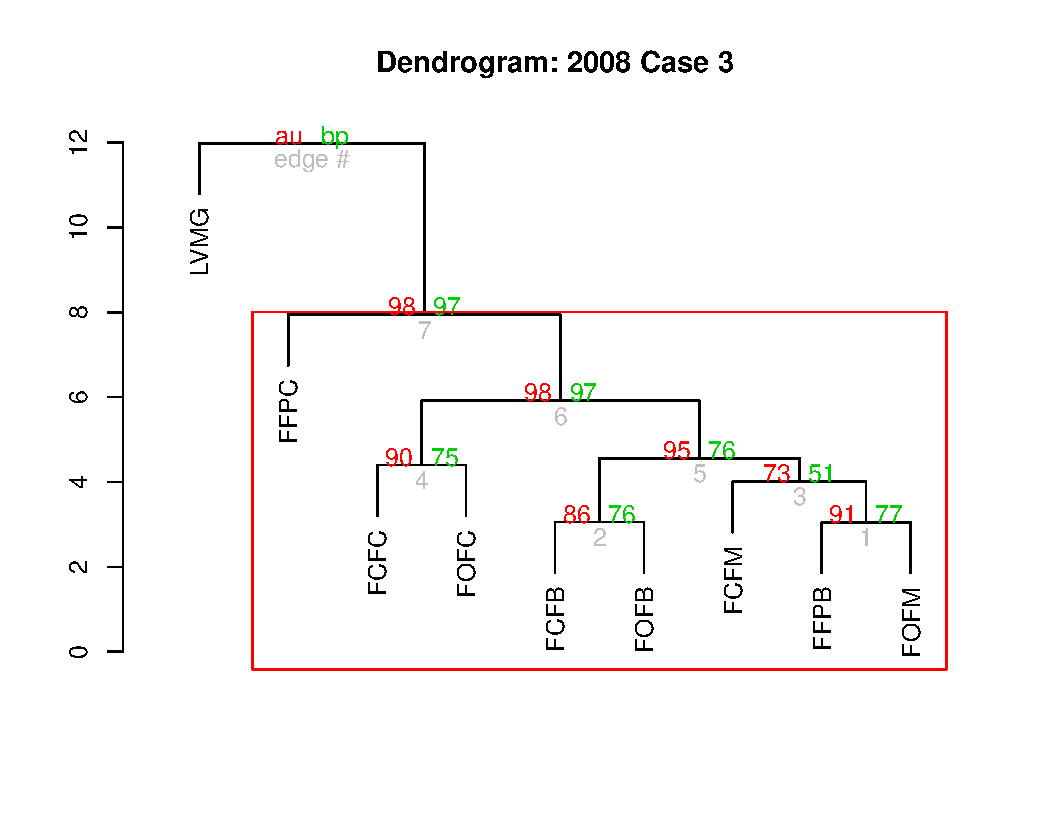
\includegraphics[width=\textwidth]{fig_dendrogram-2008-case3.pdf}
		\caption[Case 3 cluster dendrograms.]{2008 Case 3}
		\label{fig: result-fig4.10b}
	\end{subfigure}\\
	\vspace{15pt}
	\begin{subfigure}[t]{0.49\textwidth}
		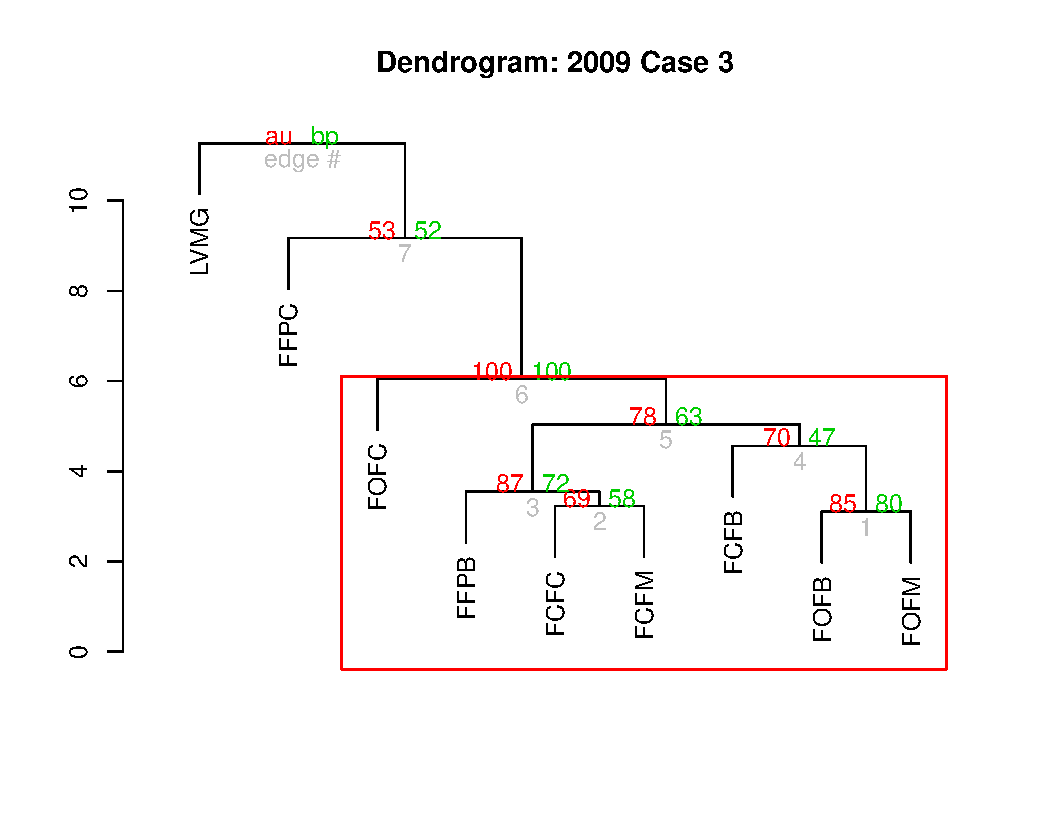
\includegraphics[width=\textwidth]{fig_dendrogram-2009-case3.pdf}
		\caption[Case 3 cluster dendrograms.]{2009 Case 3}
		\label{fig: result-fig4.10c}
	\end{subfigure}
	\begin{subfigure}[t]{0.49\textwidth}
		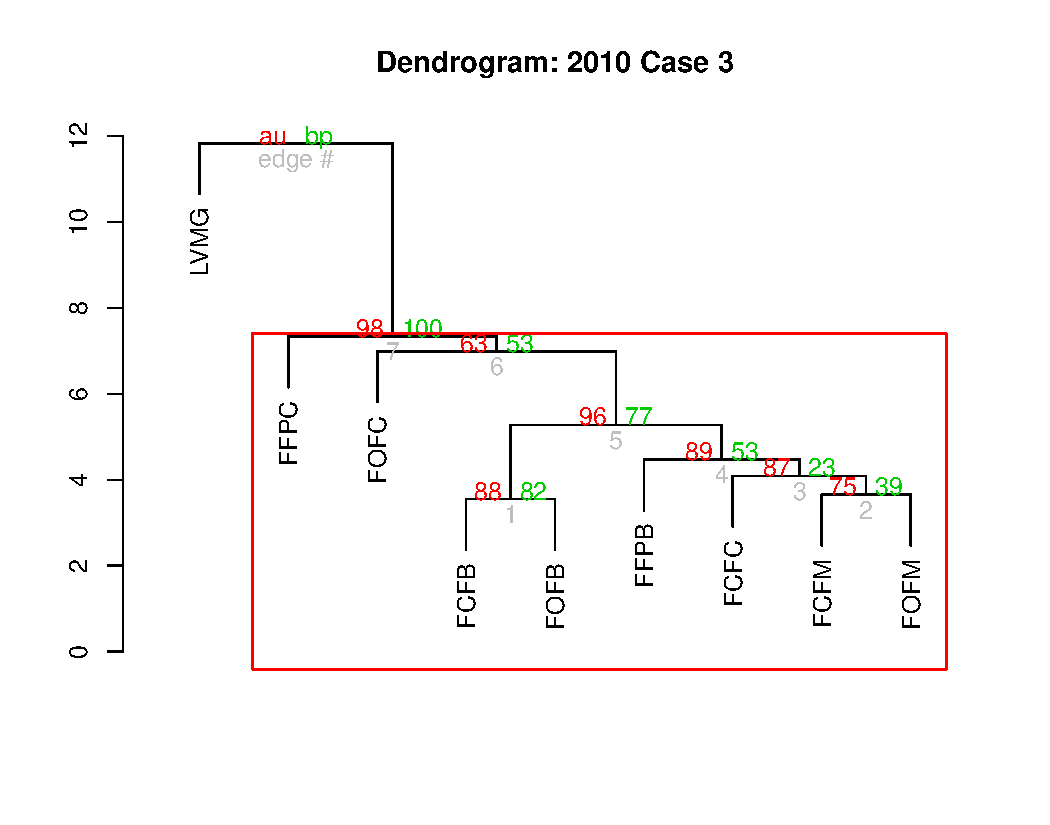
\includegraphics[width=\textwidth]{fig_dendrogram-2010-case3.pdf}
		\caption[Case 3 cluster dendrograms.]{2010 Case 3}
		\label{fig: result-fig4.10d}
	\end{subfigure}
	\vspace{5pt}
	\caption[Dendrograms from cluster analysis using Case 3.]{Dendrograms from cluster analysis using Case 3. Red boxes AU p-value $\geq$ 0.95.}
	\label{fig: result-fig4.10}
\end{figure}

\begin{figure}[!ht] \centering
	\captionsetup[subfigure]{width=2.0in} % <-- Use this to control text which is poorly spaced under a subfigure. 
	\begin{subfigure}[t]{0.49\textwidth}
		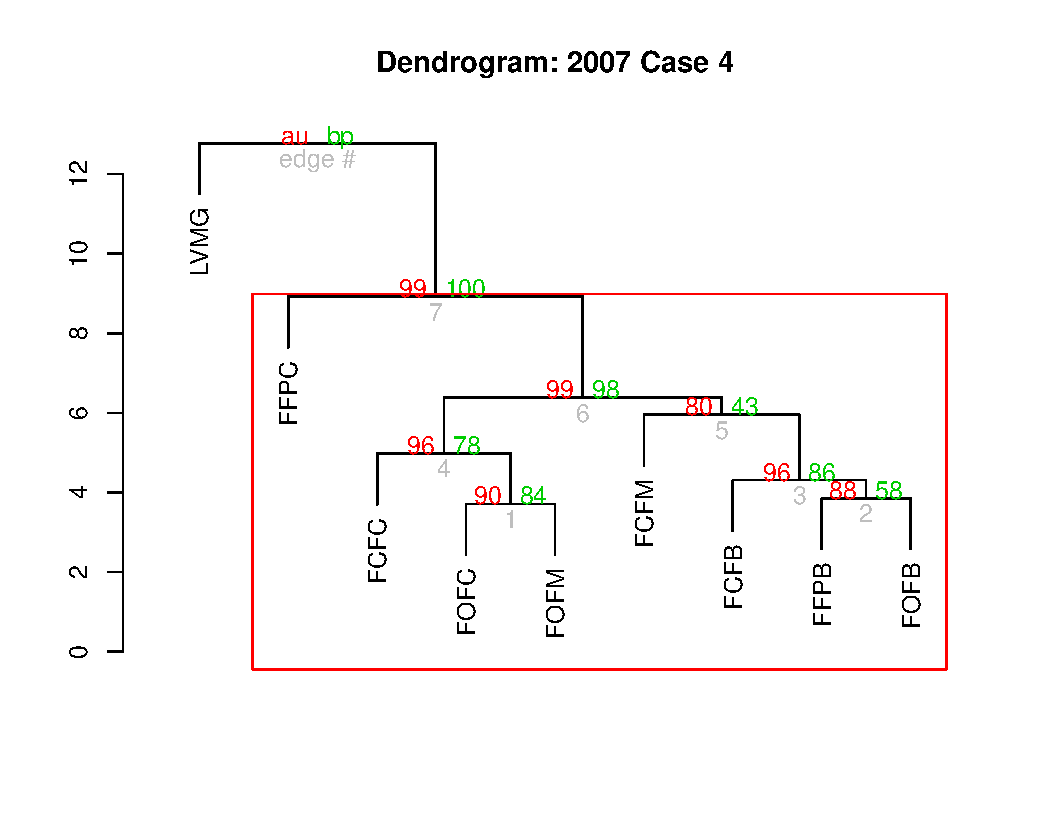
\includegraphics[width=\textwidth]{fig_dendrogram-2007-case4.pdf}
		\caption[Case 4 cluster dendrograms.]{2007 Case 4}
		\label{fig: result-fig4.11a}
	\end{subfigure}
	\begin{subfigure}[t]{0.49\textwidth}
		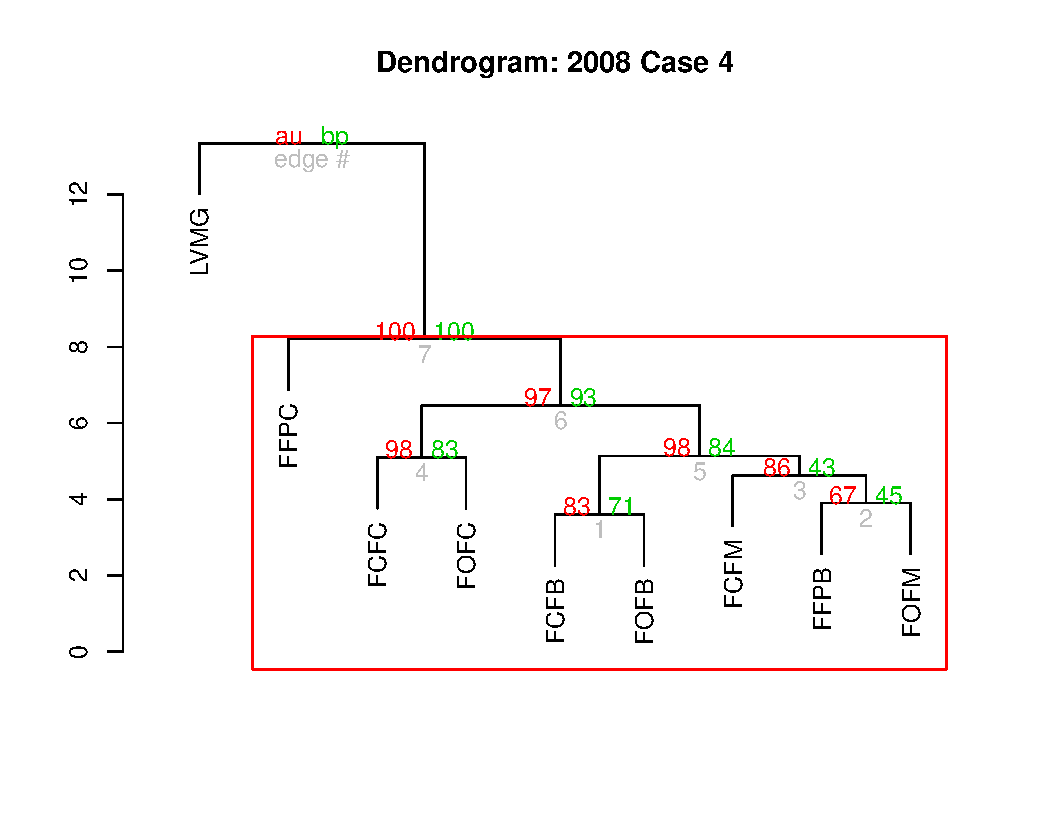
\includegraphics[width=\textwidth]{fig_dendrogram-2008-case4.pdf}
		\caption[Case 4 cluster dendrograms.]{2008 Case 4}
		\label{fig: result-fig4.11b}
	\end{subfigure}\\
	\vspace{15pt}
	\begin{subfigure}[t]{0.49\textwidth}
		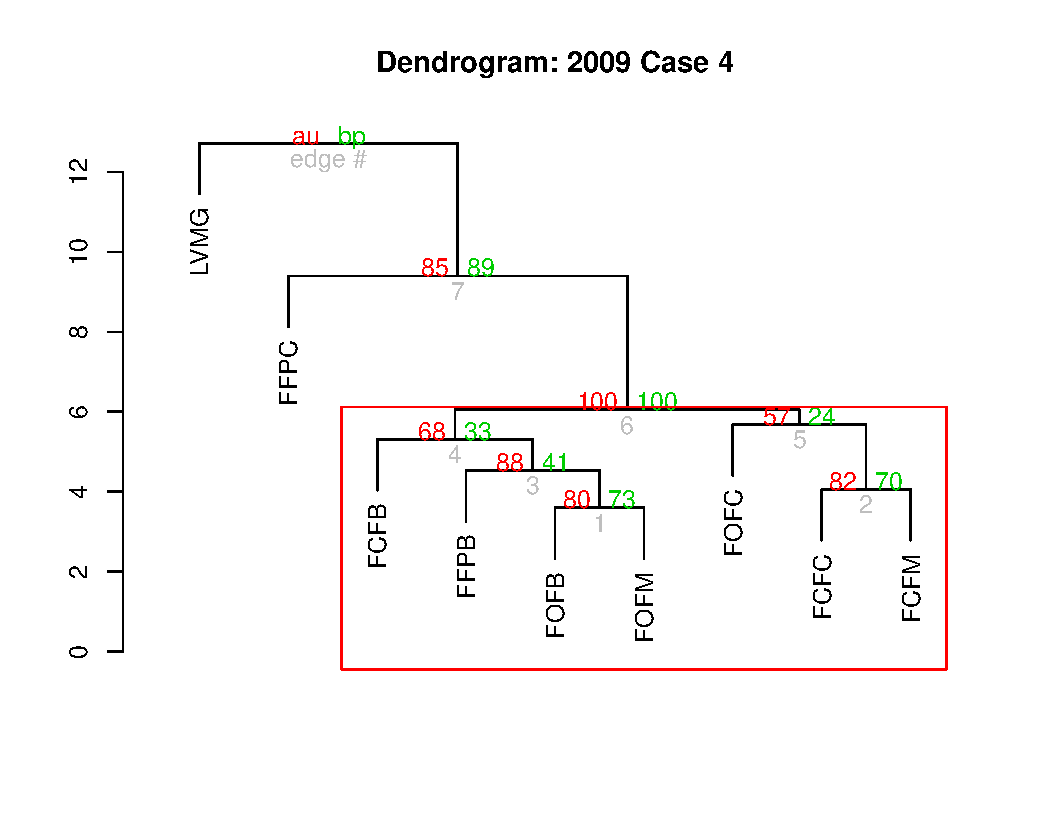
\includegraphics[width=\textwidth]{fig_dendrogram-2009-case4.pdf}
		\caption[Case 4 cluster dendrograms.]{2009 Case 4}
		\label{fig: result-fig4.11c}
	\end{subfigure}
	\begin{subfigure}[t]{0.49\textwidth}
		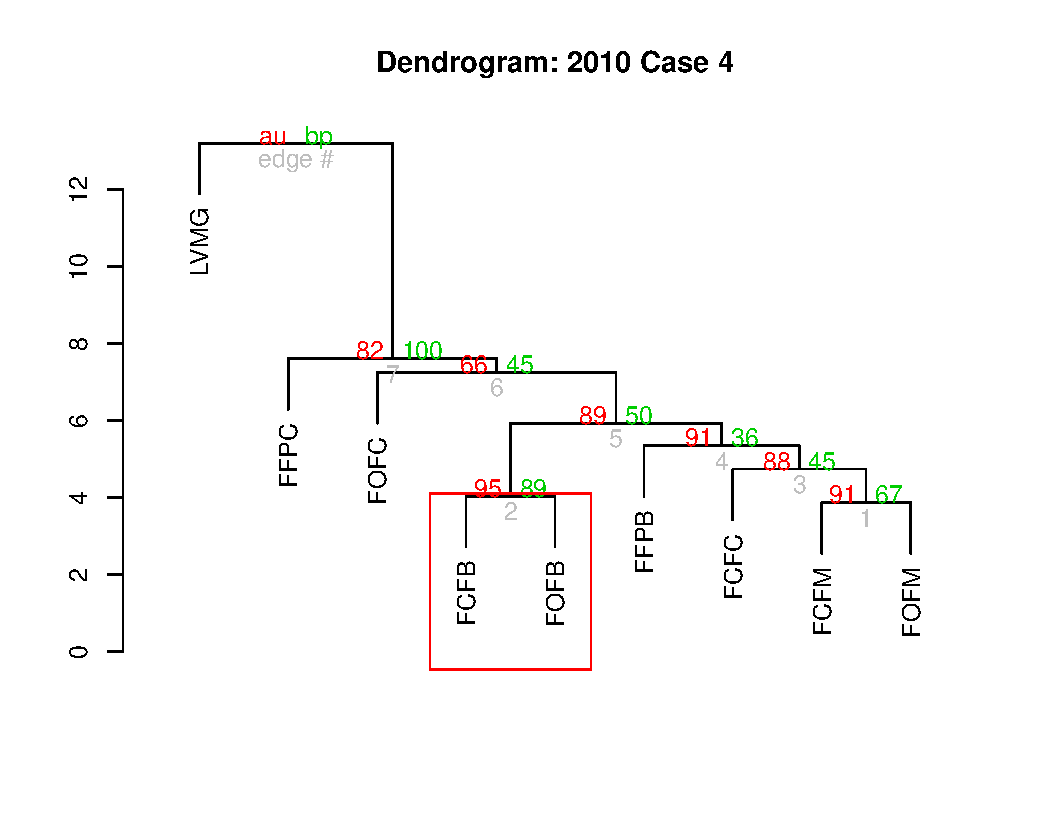
\includegraphics[width=\textwidth]{fig_dendrogram-2010-case4.pdf}
		\caption[Case 4 cluster dendrograms.]{2010 Case 4}
		\label{fig: result-fig4.11d}
	\end{subfigure}
	\vspace{5pt}
	\caption[Dendrograms from cluster analysis using Case 4.]{Dendrograms from cluster analysis using Case 4. Red boxes AU p-value $\geq$ 0.95.}
	\label{fig: result-fig4.11}
\end{figure}

\section{Accuracy of multi-level hierarchical classification approach}
\label{sec: result-accuracy-hierarchical}

Classification trees were generated for all cases or combinations of feature attributes for all years (Appendix \ref{app: appendix-trees-graphs}). For each case, 11 trees were generated from running the decision tree classification in each year, totalling 44 classification trees for one case across four years. Each tree corresponds to one of 11 classification levels based on the multi- level classification hierarchy, of which is defined by a chosen cluster dendrogram (discussed later).

An example of the generated classification trees is shown in Fig. \ref{fig: result-fig4.12} (from Appendix \ref{app: appendix-trees-graphs}), which shows four classification trees corresponding to the first four classification levels at Case 1 of the 2007 PALSAR mosaic image. Classification Level 1 splits into either Land or Water classes. Then at Level 2, with the Water class set aside, the Land class was split into either Vegetation or Non-Vegetation classes. At Level 3, the Vegetation class was split into either Forest or Non-Forest classes while the Non- Vegetation class was set aside. For Level 4, with the Non-Forest class set aside, the Forest class was split into either Mangrove forest or the other forest types group (here denoted as Forest Group 7). To interpret the classification tree, the data is split starting at top level of the tree, in this case looking at Level 1 classification tree as an example. The tree is split into two branches using Mean HH as the predictor variable, of which values less than -10.6321 in HH backscatter are assigned into the left branch, and those greater than this value are assigned into the right branch. Considering the left branch first, it is then subsequently split again into two branches again using Mean HV as the predictor variable. In this case, however, regardless whether the values are less than or greater than -20.2073 in HV backscatter, these are assigned into the Water class, which are the terminal nodes. Next, considering the right branch from the topmost node, it is split using Mean HV as the predictor variable, of which values less than -13.8405 in HV backscatter are assigned into the left branch, and those greater than this value are assigned into the right branch. Again, treating the left branch first, it is split using SD of HV layer with values less than 1.78303 assigned into the Land class and those greater than this value are assigned into the Water class, which are also both terminal nodes. Lastly, treating the right branch, it is split using Mean HV as the predictor variable. Again in this case, regardless of whether the values are less than or greater than -12.7619 in HV backscatter, these are assigned into the Land class. Once the data in Level 1 are all assigned into either the Land or Water classes, the Water class are set aside, and the data assigned to the Land class are then classified using the Level 2 classification tree, splitting into either Vegetation or Non-Vegetation classes. The classification process continues until all the data are assigned to classes ending at the Level 11 classification tree.

\begin{figure}[!ht] \centering
	\captionsetup[subfigure]{width=2.0in} % <-- Use this to control text which is poorly spaced under a subfigure. 
	\begin{subfigure}[t]{0.49\textwidth}
		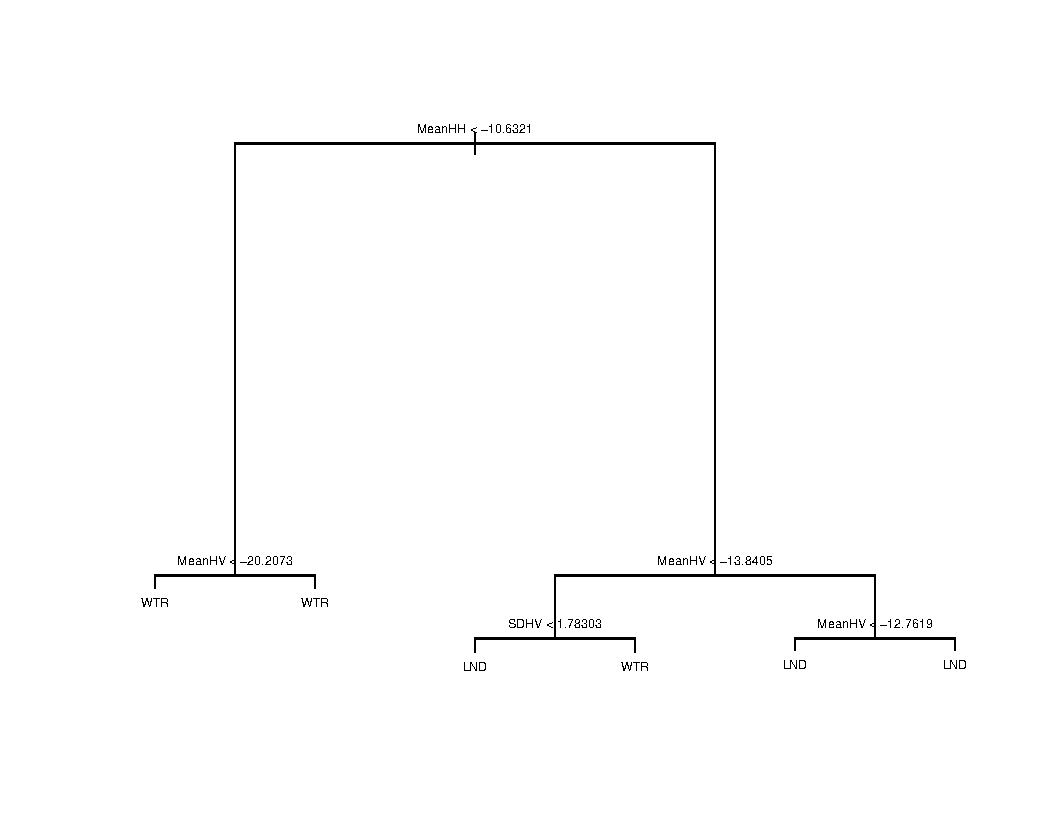
\includegraphics[width=\textwidth]{box_2007-pruned-dendrogram-lc1.pdf}
		\caption[Box.4]{Level 1}
		\label{fig: result-fig4.12a}
	\end{subfigure}
	\begin{subfigure}[t]{0.49\textwidth}
		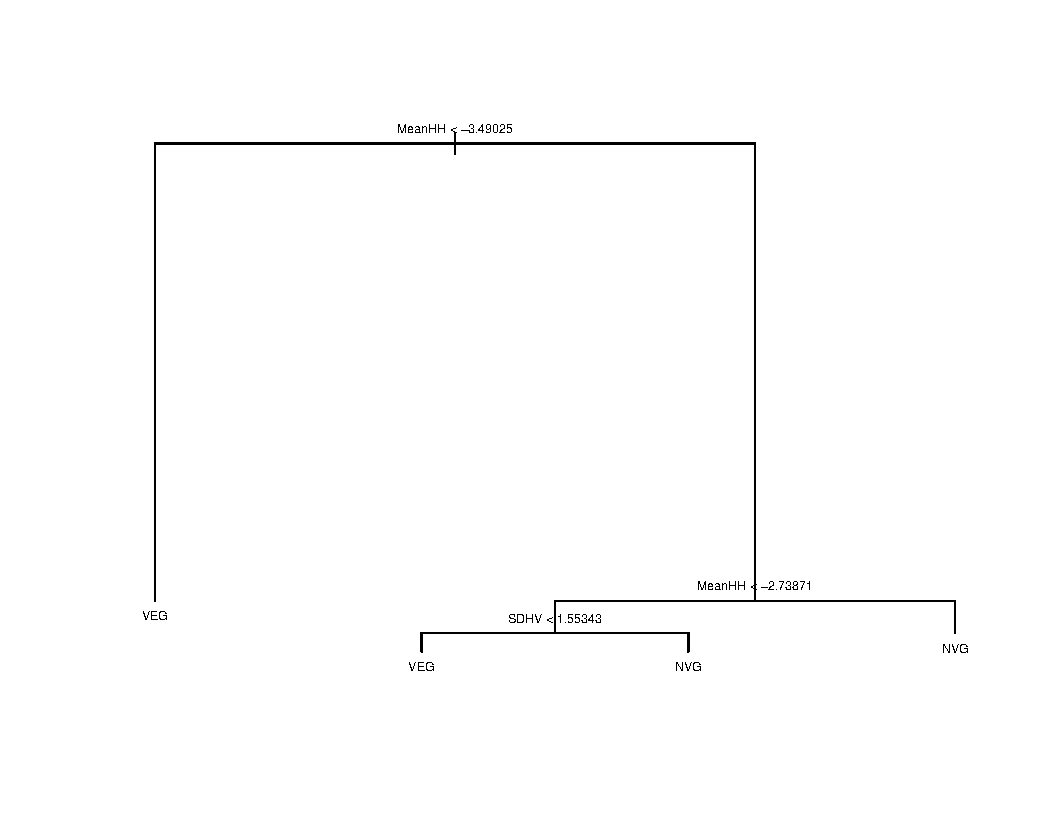
\includegraphics[width=\textwidth]{box_2007-pruned-dendrogram-lc2.pdf}
		\caption[Box.4]{Level 2}
		\label{fig: result-fig4.12b}
	\end{subfigure}\\
	\vspace{15pt}
	\begin{subfigure}[t]{0.49\textwidth}
		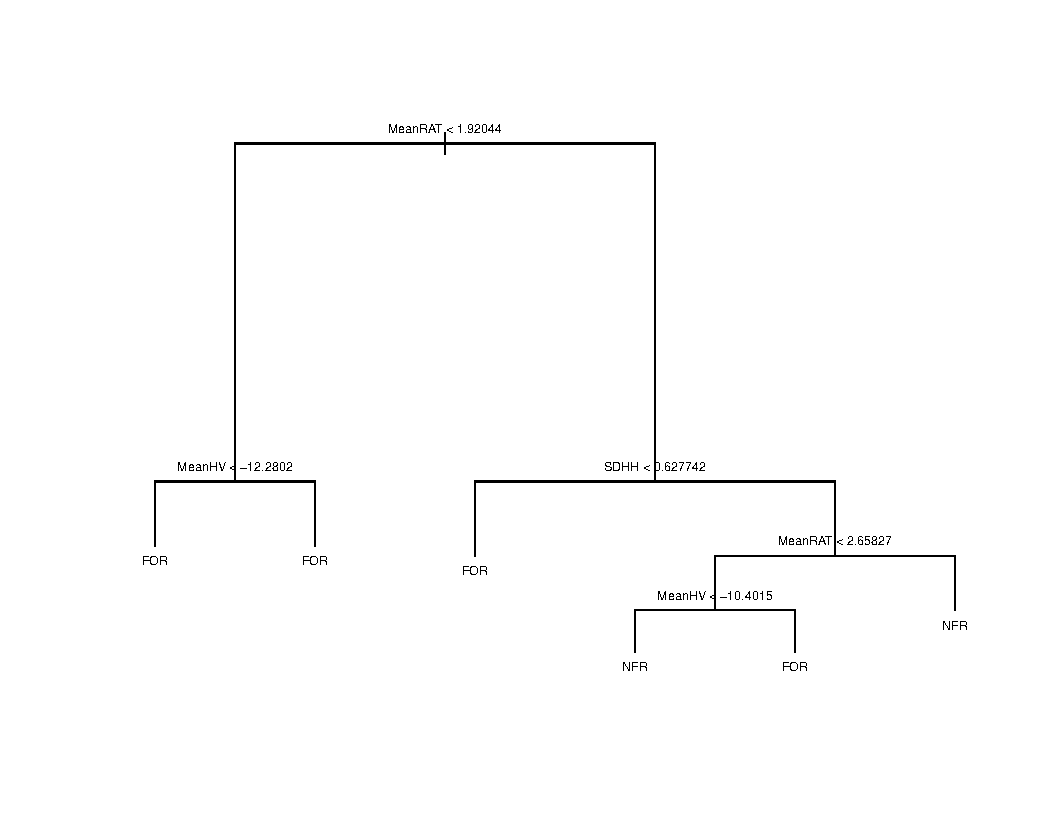
\includegraphics[width=\textwidth]{box_2007-pruned-dendrogram-lc3.pdf}
		\caption[Box.4]{Level 3}
		\label{fig: result-fig4.12c}
	\end{subfigure}
	\begin{subfigure}[t]{0.49\textwidth}
		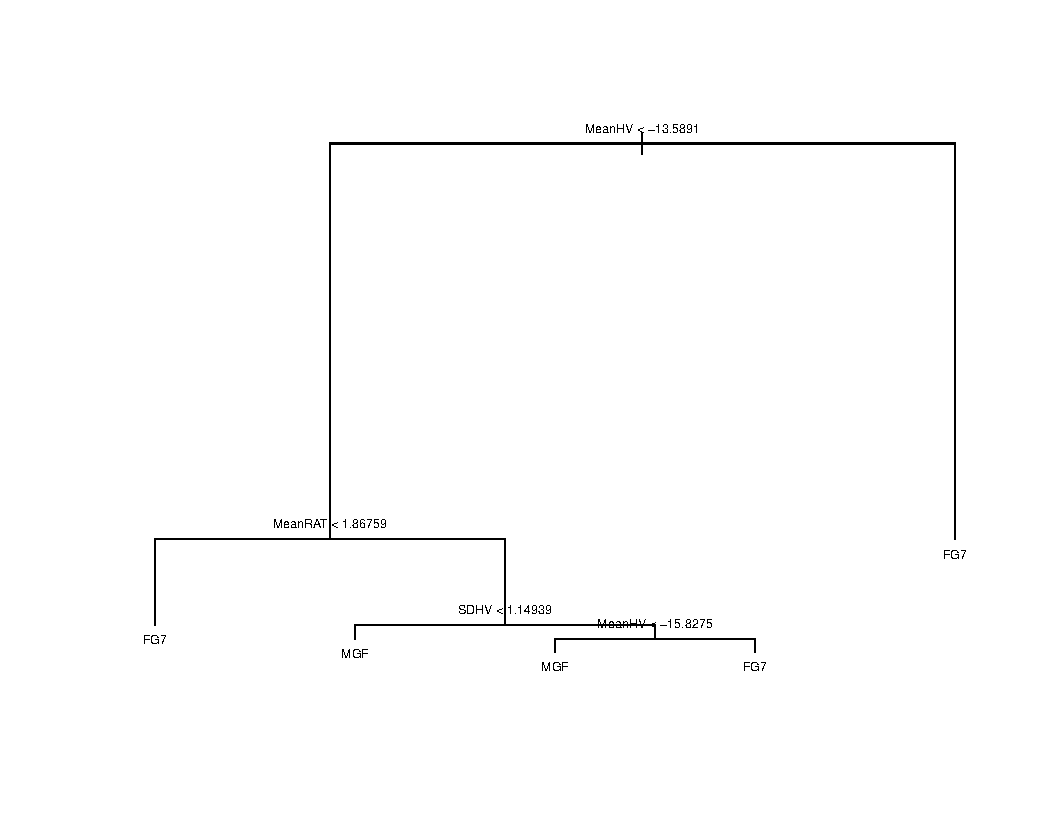
\includegraphics[width=\textwidth]{box_2007-pruned-dendrogram-lc4.pdf}
		\caption[Box.4]{Level 4}
		\label{fig: result-fig4.12d}
	\end{subfigure}
	\vspace{5pt}
	\caption[Box 4. Example classification trees corresponding to the first four classification levels at Case 1 of the 2007 PALSAR mosaic image.]{Example classification trees corresponding to the first four classification levels at Case 1 of the 2007 PALSAR mosaic image. Shown are Level 1 (land-water), Level 2 (vegetation - non-vegetation), Level 3 (forest - non-forest), and Level 4 (mangrove - non-mangrove).}
	\label{fig: result-fig4.12}
\end{figure}

The error rates obtained at each classification level per case per year were tabulated (Appendix \ref{app: appendix-error-rates}). Two sets of plots were generated: the first set of plots presented per case compared the error rates obtained for each year across classification levels (Fig. \ref{fig: result-fig4.13}); the second set of plots presented per year compared the error rates for each case across classification levels (Fig. \ref{fig: result-fig4.14}).

In Fig. \ref{fig: result-fig4.13}, the misclassification error rates across all years for all cases followed a consistent trend from classification levels 1 to 5, and turned erratic with no clear trend from classification level 6 onwards. Error rates at the first two classification levels were consistently very low across all years, indicating the suitability of PALSAR mosaics for discriminating between Land and Water (Level 1) and Vegetation and Non-Vegetation (Level 2), and this consistency was observed for multi-year PALSAR mosaics.

At Level 1, error rates decreased from Case 1 to Case 4, of which Case 4 had the lowest error rates, suggesting that the inclusion of topographic, texture, or both in addition to polarimetric variables improved classification accuracy. At Level 2, Case 2 and Case 4 showed lower error rates compared to the other two cases, suggesting that inclusion of topographic variables (Case 2) or all variables (Case 4) resulted in better separation of Vegetation and Non-Vegetation classes. Between Case 2 and Case 4, however, no significant differences in error rates were observed, suggesting that the addition of topographic variables (Case 2) or topographic and texture (Case 4) to polarimetric variables can produce the same result. At Level 3, Case 2 and Case 4 also showed lower error rates compared to the other two cases, suggesting the inclusion again of topographic variables or all variables can provide better discrimination of Forest and Non-Forest classes. At Level 4, mangrove forest (LVMG) was consistently separated from the other forest types across all cases and across all years. Notably, error rates at Level 4 resulted into zero for cases that involved topographic attributes, particularly at Case 2 and Case 4, which was primarily due to elevation—and nothing else—as the most parsimonious variable that discriminated mangroves from other forest types (Appendix \ref{app: appendix-error-rates}). This indicates that the decision tree classifier selected elevation as a determining variable for classifying mangrove forests, which is true since mangroves are situated on low elevations. However, elevation as the sole variable determining the classification of mangroves is not feasible as not all areas on low elevation are mangroves. Case 1 and Case 3 both showed low error rates in discriminating between mangrove forest and other forest types. Between the two cases, Case 3 showed slightly lower error rates compared to Case 1 suggesting that adding texture variables to polarimetric variables can marginally improve the classification accuracy. At Level 5, open canopy coniferous forest (FOFC) was consistently discriminated from other forest types in Case 1 across all years. In Case 2, closed canopy broadleaved forest (FCFB) was consistently discriminated from other forest types across all years. For Case 3 and Case 4, coniferous forest plantation (FFPC) was consistently discriminated from other forest types across all years. This particular discrimination of one forest type from the others may suggest the influence of specific predictor variables (or combinations thereof) for discriminating these forest types at this classification level. Finally, for Level 6 onwards, no apparent trend was observed except the erratic behaviour of the graphs of error rates, suggesting the varied influence of predictor variables at specific cases in the discrimination of forest types.

In Fig. \ref{fig: result-fig4.14}, the misclassification error rates were presented this time per year to compare each case across classification levels. Similar to Fig. \ref{fig: result-fig4.13}, error rates across all cases for all years followed a consistent trend from classification levels 1 to 5, and turned erratic with no clear trend from classification level 6 onwards. The error rates at the first two classification levels, specifically Level 1 (Land and Water) and Level 2 (Vegetation and Non-Vegetation) were consistently very low across cases for all years. The error rates spiked at Level 3 (Forest and Non-Forest) for all cases, of which Case 2 and Case 4 exhibited the lower error rates compared to the other cases (Appendix \ref{app: appendix-error-rates}), and subsequently Case 4 had the lowest error rates compared to Case 2. At Level 4, error rates were low for Case 1 and Case 3, and resulted to 0 for Case 2 and 4. At Level 5, Case 1 and 2 showed higher error rates compared to the other two cases across all years.\\

\begin{figure}[!ht] \centering
	\captionsetup[subfigure]{width=2.0in} % <-- Use this to control text which is poorly spaced under a subfigure. 
	\begin{subfigure}[t]{0.49\textwidth}
		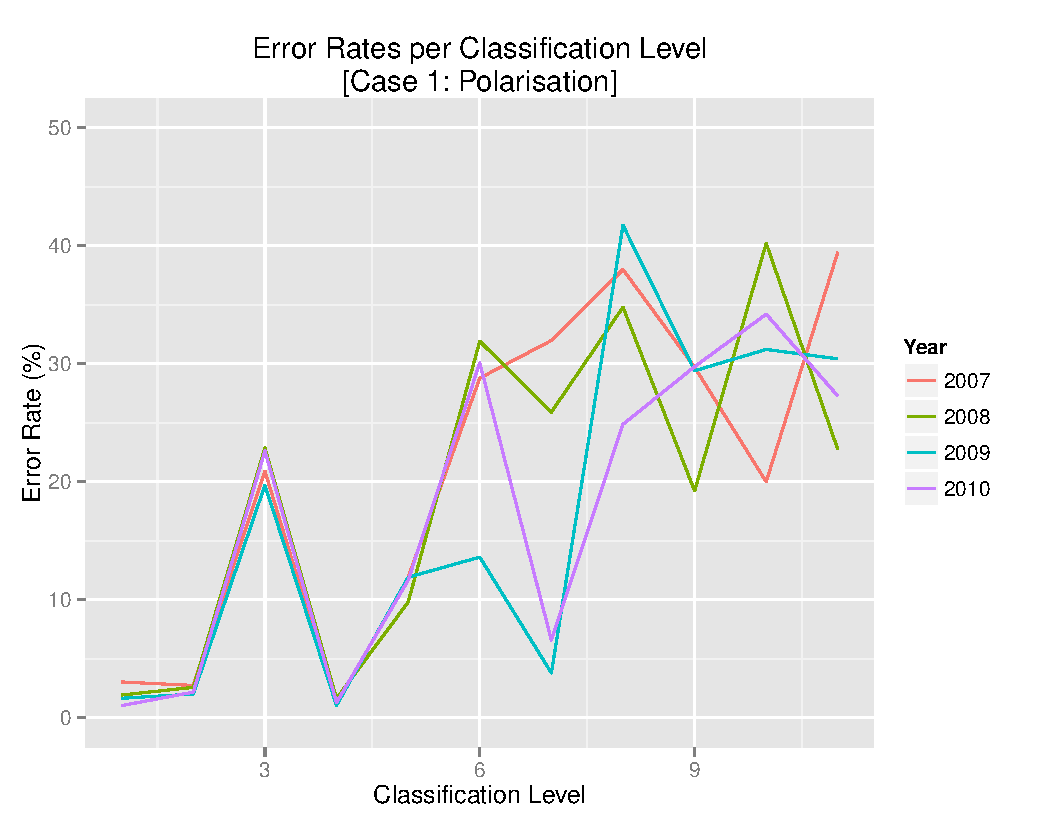
\includegraphics[width=\textwidth]{fig_graph-pruned-case1.pdf}
		\caption[Error rates across levels per case.]{Case 1}
		\label{fig: result-fig4.13a}
	\end{subfigure}
	\begin{subfigure}[t]{0.49\textwidth}
		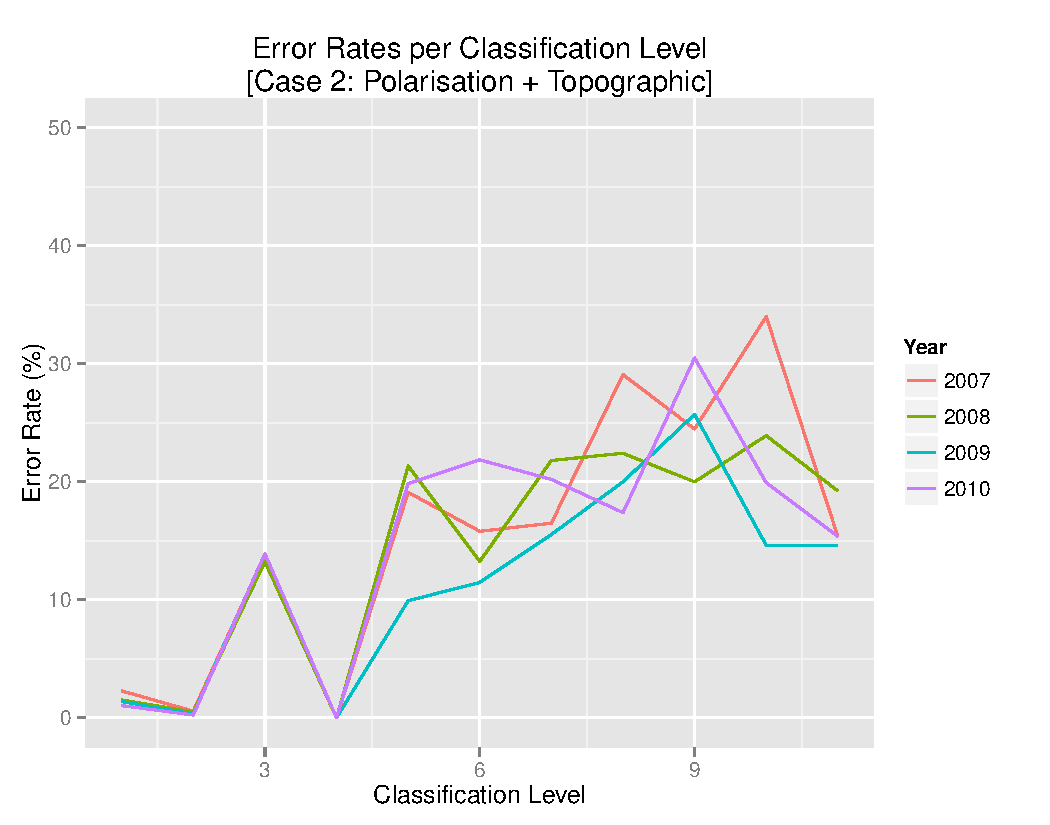
\includegraphics[width=\textwidth]{fig_graph-pruned-case2.pdf}
		\caption[Error rates across levels per case.]{Case 2}
		\label{fig: result-fig4.13b}
	\end{subfigure}\\
	\vspace{15pt}
	\begin{subfigure}[t]{0.49\textwidth}
		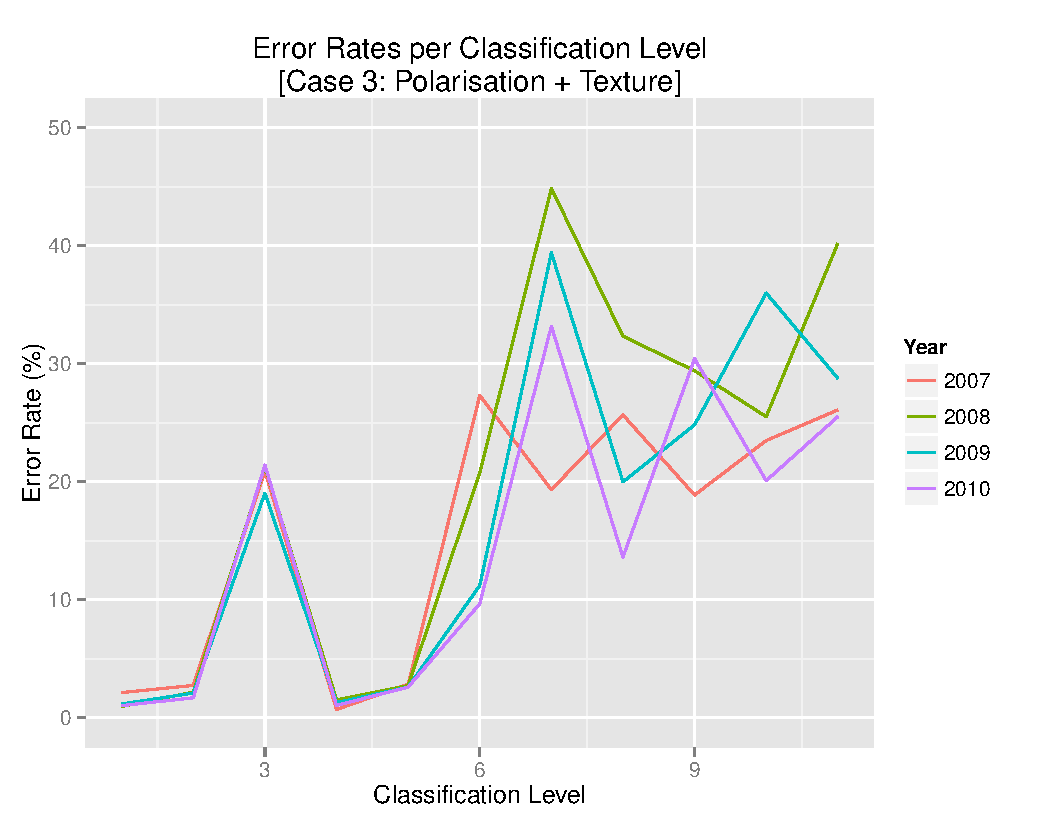
\includegraphics[width=\textwidth]{fig_graph-pruned-case3.pdf}
		\caption[Error rates across levels per case.]{Case 3}
		\label{fig: result-fig4.13c}
	\end{subfigure}
	\begin{subfigure}[t]{0.49\textwidth}
		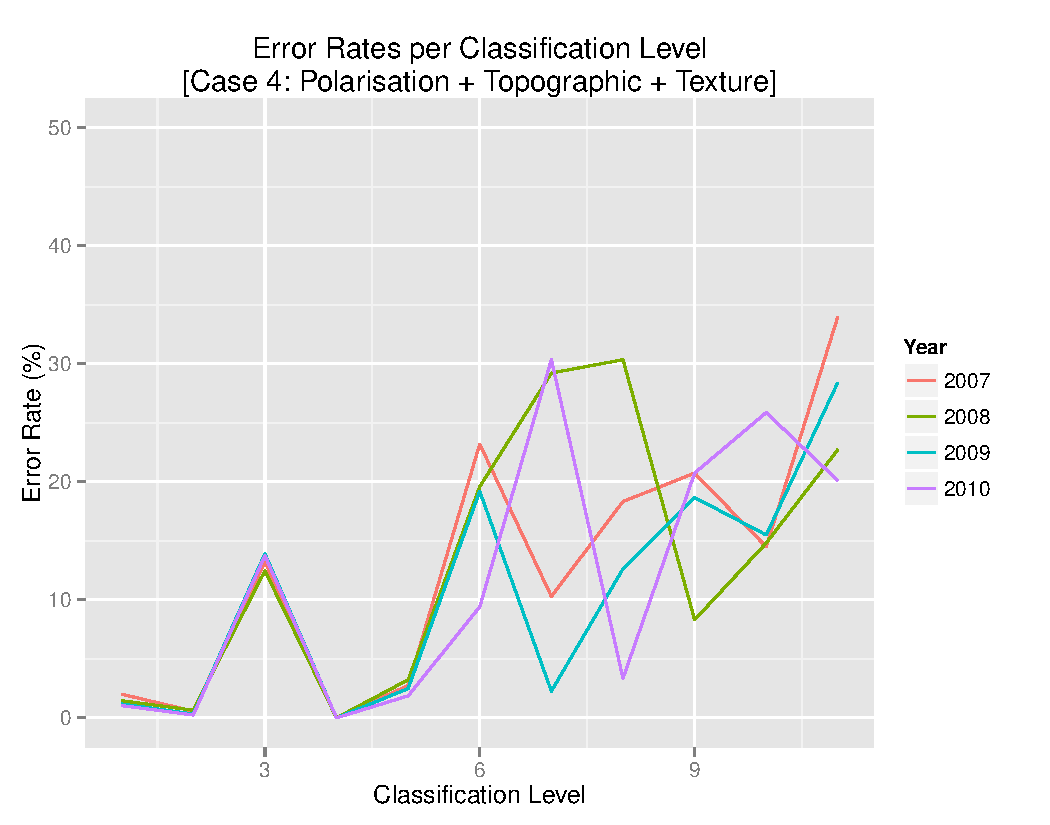
\includegraphics[width=\textwidth]{fig_graph-pruned-case4.pdf}
		\caption[Error rates across levels per case.]{Case 4}
		\label{fig: result-fig4.13d}
	\end{subfigure}
	\vspace{5pt}
	\caption[Plots comparing error rates obtained for each year across classification levels per case.]{Plots comparing error rates obtained for each year across classification levels per case.}
	\label{fig: result-fig4.13}
\end{figure}

\begin{figure}[!ht] \centering
	\captionsetup[subfigure]{width=2.0in} % <-- Use this to control text which is poorly spaced under a subfigure. 
	\begin{subfigure}[t]{0.49\textwidth}
		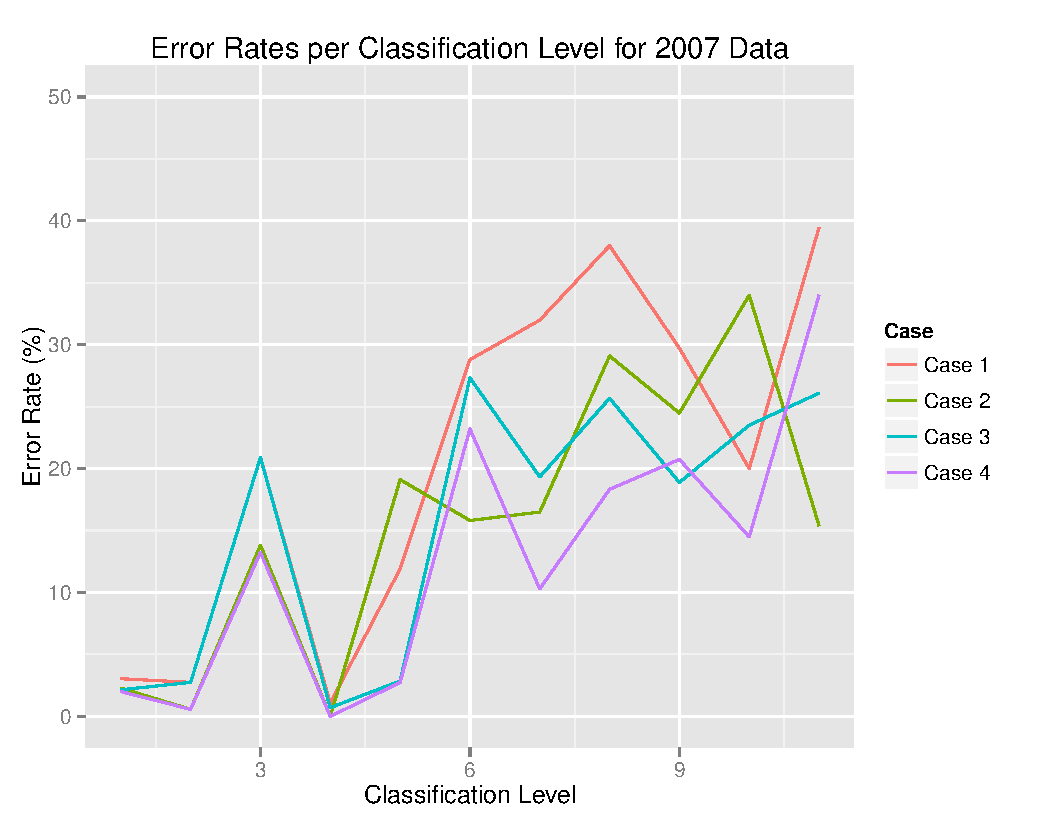
\includegraphics[width=\textwidth]{fig_graph-pruned-2007.pdf}
		\caption[Error rates across levels per year.]{2007}
		\label{fig: result-fig4.14a}
	\end{subfigure}
	\begin{subfigure}[t]{0.49\textwidth}
		\includegraphics[width=\textwidth]{fig_graph-pruned-2008.pdf}
		\caption[Error rates across levels per year.]{2008}
		\label{fig: result-fig4.14b}
	\end{subfigure}\\
	\vspace{15pt}
	\begin{subfigure}[t]{0.49\textwidth}
		\includegraphics[width=\textwidth]{fig_graph-pruned-2009.pdf}
		\caption[Error rates across levels per year.]{2009}
		\label{fig: result-fig4.14c}
	\end{subfigure}
	\begin{subfigure}[t]{0.49\textwidth}
		\includegraphics[width=\textwidth]{fig_graph-pruned-2010.pdf}
		\caption[Error rates across levels per year.]{2010}
		\label{fig: result-fig4.14d}
	\end{subfigure}
	\vspace{5pt}
	\caption[Plots comparing error rates obtained for each case across classification levels per year.]{Plots comparing error rates obtained for each case across classification levels per year.}
	\label{fig: result-fig4.14}
\end{figure}

\begin{spacing}{1.0}
\begin{longtable}[h!]{ p{2.6cm} p{2.6cm} p{2.6cm} p{2.6cm} p{2.6cm} }

    \caption[Summary of total classification error rates per case per year.]{Summary of total classification error rates per case per year.}
    \label{tab: result-table4.3}\\
    
    	\toprule
    	Case & 2007 & 2008 & 2009 & 2010\\
    	\midrule
    	\endhead
    	
		1 & 163.745 & 158.784 & 155.709 & 160.277\\
		2 & 101.349 & 103.588 &  91.795 & 102.603\\
		3 &  95.333 & 101.463 &  98.812 &  96.342\\
		4 &  74.556 &  78.679 &  69.118 &  70.525\\
		
		\bottomrule \\
    
\end{longtable}
\end{spacing}

A subsequent summary of the total classification error rates per case per year was computed (Table \ref{tab: result-table4.3}). The table showed that the inclusion of topographic and texture attributes (Case 2 and Case 3, respectively) tend to reduce the misclassification error rates compared to using solely polarimetric attributes (Case 1). The addition of topographic to polarimetric attributes (Case 2) also showed higher error rates compared to a polarimetric and texture combination (Case 3). The inclusion of all feature attributes (Case 4), including polarimetric, topographic, and texture, produced the lowest misclassification error rates across years; and consequently, it formed the bases of the classification hierarchies that were constructed through rulesets to produce the annual land cover maps (Fig. \ref{fig: result-fig4.15}).

The mean error rates of land cover classes for each case and each year were tabulated (Table \ref{tab: result-table4.4}), which indicates that the mean error rates were still the lowest for Case 4 compared to other cases across all years. The inclusion of either topographic or texture attributes to polarimetric data tended to lower the classification error rates, of which error rates with texture included was lower compared to error rates with topographic attributes included. This emphasises that the inclusion of both topographic and texture feature attributes improve the classification accuracy of forest cover types.\\

\begin{spacing}{1.0}
\begin{longtable}[h!]{ p{2cm} p{2.7cm} p{2.7cm} p{2.7cm} p{2.9cm} }

    \caption[Summary of total classification error rates per case per year.]{Summary of total classification error rates per case per year.}
    \label{tab: result-table4.4}\\
    
    	\toprule
    	Case & 2007 & 2008 & 2009 & 2010\\
    	\midrule
    	\endhead
    	
		1 & 14.886 $\pm$ 10.04 & 14.435 $\pm$ 10.11 & 14.155 $\pm$ 12.68 & 14.571 $\pm$ 10.870\\
		2 &  9.214 $\pm$ 6.137 &  9.417 $\pm$ 6.777 &  8.345 $\pm$ 5.221 &  9.328 $\pm$ 6.486\\
		3 &  8.667 $\pm$ 8.138 &  9.224 $\pm$ 7.618 &  8.983 $\pm$ 9.273 &  8.758 $\pm$ 8.743\\
		4 &  6.778 $\pm$ 6.458 &  7.153 $\pm$ 6.155 &  6.283 $\pm$ 5.793 &  6.411 $\pm$ 6.416\\
		
		\bottomrule \\
    
\end{longtable}
\end{spacing}

\begin{figure}[!ht] \centering
	\captionsetup[subfigure]{width=2.0in} % <-- Use this to control text which is poorly spaced under a subfigure. 
	\begin{subfigure}[t]{0.49\textwidth}
		\includegraphics[width=\textwidth]{fig_classification-2007.jpg}
		\caption[Land cover and forest type maps.]{2007}
		\label{fig: result-fig4.15a}
	\end{subfigure}
	\begin{subfigure}[t]{0.49\textwidth}
		\includegraphics[width=\textwidth]{fig_classification-2008.jpg}
		\caption[Land cover and forest type maps.]{2008}
		\label{fig: result-fig4.15b}
	\end{subfigure}\\
	\vspace{10pt}
	\begin{subfigure}[t]{0.49\textwidth}
		\includegraphics[width=\textwidth]{fig_classification-2009.jpg}
		\caption[Land cover and forest type maps.]{2009}
		\label{fig: result-fig4.15c}
	\end{subfigure}
	\begin{subfigure}[t]{0.49\textwidth}
		\includegraphics[width=\textwidth]{fig_classification-2010.jpg}
		\caption[Land cover and forest type maps.]{2010}
		\label{fig: result-fig4.15d}
	\end{subfigure}\\
	\vspace{10pt}
	\begin{subfigure}[t]{0.25\textwidth}
		\includegraphics[width=\textwidth]{fig_classification-legend.png}
		\caption[Land cover and forest type maps.]{Legend}
		\label{fig: result-fig4.15e}
	\end{subfigure}
	\vspace{5pt}
	\caption[Land cover and forest type maps generated from annual ALOS/PALSAR mosaics using decision tree classification.]{Land cover and forest type maps generated from annual ALOS/PALSAR mosaics using decision tree classification.}
	\label{fig: result-fig4.15}
\end{figure}

\section{Accuracy of heuristic classification approach}
\label{sec: result-accuracy-heuristic}

Additional assessments of classification accuracies were done to discriminate: (a) closed and open canopy forests; and (b) broadleaved, coniferous, and mixed forests through a heuristic approach without following the hierarchical clustering result. It should be noted here that the error rates obtained for the first four classification levels for both groups were the same values obtained in the previous sub-section.

\subsection{Closed and open canopy forests}

The final classification level at Level 5 dealt with separating closed canopy and open canopy forests, of which each group consisted of the following specific forest types: for closed canopy forests, the forest types included closed broadleaved (FCFB), closed coniferous (FCFC), and closed mixed (FCFM); for open canopy forests, the forest types included open broadleaved (FOFB), open coniferous (FOFC), open mixed (FOFM), broadleaved forest plantation (FFPB), and coniferous forest plantation (FFPC).\\

\begin{spacing}{1.0}
\begin{longtable}[h!]{ p{2.6cm} p{2.6cm} p{2.6cm} p{2.6cm} p{2.6cm} }

    \caption[Classification error rates for closed and open canopy forests per case per year using a heuristic approach.]{Classification error rates for closed and open canopy forests per case per year using a heuristic approach.}
    \label{tab: result-table4.5}\\
    
    	\toprule
    	Case & 2007 & 2008 & 2009 & 2010\\
    	\midrule
    	\endhead
    	
		1 & 36.35 & 37.22 & 37.22 & 35.24\\
		2 & 30.89 & 32.13 & 29.90 & 29.40\\
		3 & 36.35 & 37.22 & 37.22 & 35.24\\
		4 & 30.89 & 32.13 & 32.13 & 29.40\\
		
		\bottomrule \\
    
\end{longtable}
\end{spacing}

Results showed that error rates at Level 5 were exactly the same in Case 1 and Case 3, and almost the same for Case 2 and Case 4 with the exception of values in 2009 (Table \ref{tab: result-table4.5}). Error rates in Case 1 and Case 3 were similar, suggesting that texture variables do not contribute to improving classification accuracy in discriminating between closed and open canopy forests. Case 2 and Case 4 showed lower error rates compared to the other two cases, suggesting that topographic variables contributed to improving classification accuracy in discriminating between closed and open canopy forests by 5-7\%. Overall, classification error rates at Level 5 were high at approximately 29-38\%.

\subsection{Broadleaved, coniferous, and mixed forests}

The final classification level at Level 5 dealt with separating broadleaved, coniferous, and mixed forests, of which each group consisted of the following specific forest types: broadleaved forests included closed broadleaved (FCFB), open broadleaved (FOFB), and broadleaved forest plantation (FFPB); coniferous forests included closed coniferous (FCFC), open coniferous (FOFC), and coniferous forest plantation (FFPC); and mixed forests included closed mixed (FCFM) and open mixed (FOFM).\\

\begin{spacing}{1.0}
\begin{longtable}[h!]{ p{2.6cm} p{2.6cm} p{2.6cm} p{2.6cm} p{2.6cm} }

    \caption[Classification error rates for closed and open canopy forests per case per year using a heuristic approach.]{Classification error rates for closed and open canopy forests per case per year using a heuristic approach.}
    \label{tab: result-table4.6}\\
    
    	\toprule
    	Case & 2007 & 2008 & 2009 & 2010\\
    	\midrule
    	\endhead
    	
		1 & 43.42 & 44.04 & 41.44 & 41.19\\
		2 & 32.26 & 33.37 & 33.25 & 31.89\\
		3 & 43.42 & 44.04 & 41.44 & 41.19\\
		4 & 32.26 & 33.37 & 33.25 & 33.75\\
		
		\bottomrule \\
    
\end{longtable}
\end{spacing}

Results showed that classification error rates at Level 5 were exactly the same in Case 1 and Case 3, and almost the same for Case 2 and Case 4 with the exception of values in 2010 (Table \ref{tab: result-table4.6}). Error rates in Case 1 and Case 3 were similar, suggesting that texture variables do not contribute to improving classification accuracy in discriminating between broadleaved, coniferous, and mixed forests. Case 2 and Case 4 showed lower error rates compared to the other two cases, suggesting that topographic variables contributed to improving classification accuracy in discriminating between broadleaved, coniferous, and mixed forests by 8-11\%. Overall, classification error rates at Level 5 were high at approximately 31-44\%, of which were also higher compared to error rates obtained in classifying between closed and open canopy forests (Table \ref{tab: result-table4.5}).

\subsection{Area statistics of land cover types}

The area statistics of each land cover type was computed from the resulting land cover maps from the decision tree classification of multi-year PALSAR mosaics, specifically based on Case 4 (utilising all predictor variables, namely polarimetric, topographic, and texture) from the hierarchical clustering approach (Table \ref{tab: result-table4.7}).

Significant differences can be seen from the area figures across years for all land cover types. This may be attributed to the high error rates, specifically in the classification of different forest types. Differences in area statistics can also be observed between figures obtained from the PALSAR mosaics and the NAMRIA 2010 land cover map. (Note that differences in total area figures at the bottom row may be attributed to masked areas in the PALSAR mosaics due to shadow and layover.)\\

\begin{spacing}{1.0}
\begin{longtable}[h!]{ p{3cm} p{2cm} p{2cm} p{2cm} p{2cm} p{2cm} }

    \caption[Area statistics of land cover types from classified annual PALSAR mosaics.]{Area statistics of land cover types from classified annual PALSAR mosaics.}
    \label{tab: result-table4.7}\\
    
    	\toprule
    	Class & {} & {} & PALSAR & {} & NAMRIA\\
    	\cmidrule{2-6}
    	{} & 2007 (ha) & 2008 (ha) & 2009 (ha) & 2010 (ha) & 2010 (ha)\\ 
    	\midrule
    	\endhead
    	
		Water & 634,067 & 461,769 & 345,434 & 349,074 & {}\\
		Non-vegetation & 376,640 & 421,192 & 302,471 & 114,440 & {}\\
		Non-forest & 805,576 & 1,670,234 & 1,526,462 & 1,851,864 & 3,085,588\\
		Mangrove forest & 183,238 & 90,844 & 151,386 & 88,734 & 2,122\\
		CFB & 4,045 & 42,453 & 127,200 & 104,958 & 685,677\\
		CFC & 9,556 & {} & 106,556 & 144,578 & 15,905\\
		CFM & 124,515 & 258,253 & 101,324 & 209,390 & 26,072\\
		OFB & 1,608,354 & 616,830 & 1,531,202 & 1,065,904 & 841,185\\
		OFC & {} & 190,995 & 6,670 & 55,054 & 163,806\\
		OFM & 1,444 & 277,572 & 56,492 & 106,434 & 65,604\\
		FPB & 528,260 & 246,608 & 3,627 & 185,417 & 22,067\\
		FPC & 1,519 & 215 & 18,183 & 1,068 & 802\\
		\midrule
		Total & 4,276,915 & 4,276,915 & 4,276,915 & 4,276,915 & 4,908,828\\
		\bottomrule
    
\end{longtable}

	\noindent Note: CFB: Closed forest, broadleaved; CFC: Closed forest, coniferous; CFM: Closed forest, mixed; OFB: Open forest, broadleaved; OFC: Open forest, coniferous; OFM: Open forest, mixed; FPB: Forest plantation, broadleaved; FPC: Forest plantation, coniferous.\\
	
\end{spacing}

